\chapter{Introduction}
% My introduction - focus:
% The emphasis should be put on the last 2 layers with cursory information for the top two as needed
% Biology, biochemistry, biophysics, molecular details / simulations

% Check out Misbehaving proteins the book.

% Broad theme: Protein folding, self-assembly, and its modulation ???
% Flow of information from DNA to protein, where proteins carry out core functions which enable life.
% Importance of protein folding -- structure - function paradigm
% Functions by binding with other proteins or ligands in the body. Protein interactions and how protein function may be modulated by these interactions -- particularly solvent interactions.
% Ok, we also know about intrinsically disordered proteins that have well-defined functions in the human body.
% But what about amyloid ... this common state that all proteins reach which results from protein aggregation .. involved in disease.

One of the most remarkable phenomenon in nature is the ability of proteins to fold from a polypeptide chain into structures which impart their functions as molecular machines of life. Proteins play a key role in all aspects of life, from cell cycle regulation to signal transduction. 

% Small molecules that can affect the outcome of various biochemical pathways act by binding these protein receptors. 
%Specific examples of the molecular basis underlying certain cellular mechanisms involving protein-ligand binding
Much of the critical regulation of biological activity within a cell is mediated by receptor-ligand interactions, often in the form of binding interactions between a receptor and an inhibitory ligand. REFs
Furthermore, apoptosis (3) and autophagy (4), cellular mechanisms that are in place to prevent unregulated cell division, are also dependent on well-orchestrated receptor-ligand interactions. REFs

When these systems are dysregulated, the consequences can be devastating to the cell and/or organism. For example, disruptions to the regulation of cell cycle progression and proliferation lead to diseases such as cancer (1, 2). 
(Adapted from tummino and copeland 2008)
% Can also cite this paper
% Complement receptor ligand binding -- http://www.annualreviews.org/doi/abs/10.1146/annurev.iy.01.040183.001331?journalCode=immunol
% The cell biology of receptor-mediated virus entry -- http://jcb.rupress.org/content/195/7/1071.full
It is not surprising that many diseases arise from the improper functioning of proteins, for example, when mutations occur or when they denature or misfold (fail to adopt their native functional state). Hence, about 40\% of modern medicine targets the G protein-coupled receptors, a large protein family of receptors found in eukaryotes that sense molecules outside the cell and activate inside signal transduction pathways, and ultimately cellular responses.
% REF http://en.wikipedia.org/wiki/G_protein-coupled_receptor#Ligand_binding

% Important to understand structure, but it is not enough.  We also need to understand dynamics
Since the historical experiment performed by Anfinsen and colleagues which demonstrated that the structure of a folded protein is encoded in its amino acid sequence and solvent environment, protein folding and structure determination have gained much attention in the fields of biochemistry and biophysics.  The static models produced by NMR, X-ray crystallography, and homology modeling provide valuable insights into macromolecular structure, but molecular recognition and drug binding are very dynamic processes.  When a small molecule like a drug (for example, a ligand) approaches its target (for example, a receptor) in solution, it encounters not a single, frozen structure, but rather a macromolecule in constant motion. Understanding both protein structure and dynamics enable us to elucidate the molecular basis of disease pathways and ultimately will aid in the discovery of novel therapeutics. 

% Computer-aided drug design using MD
As ligand binding and the important macromolecular motions associated with it are microscopic events that take place in mere millionths of a second, a complete understanding of the atomistic energetics and mechanics of binding is unattainable using current experimental techniques. In recent years, molecular dynamics (MD) simulation of biomolecules, a physics-based computer simulation technique, became a tool of choice to investigate protein dynamics and function, and ligand-binding

Currently, MD simulations is the most accurate computational method for probing small-molecule binding, and are useful for filling in the details where experimental methods cannot.\cite{Durrant:2011bm} In the past few years, MD simulations are able to routinely reach microseconds in sampling time. With the ever increase in the availability of computing power and data storage, simulations are a promising technique for aiding in the structure-based drug discovery process. 
% With constant improvements in both computer algorithms and processing power, molecular dynamics simulations are likely to play an increasingly important role in the development of novel pharmacological therapeutics.\cite{Durrant:2011bm}  % [There are examples already demonstrating MD's usefulness in drug ... cite some examples from that DE Shaw paper]

% IDPs have function.  Break down of folded structure, and aggregation leads to loss of function.
% Protein misfolding and aggregation
In recent years, a class of proteins without a uniquely folded state known as intrinsically disordered proteins (IDPs) have gained attention because of their involvement in a multitude of physiological pathways and diseases.   For example, proteins associated with cell signalling and cancer in humans are predicted to be enriched in protein disorder (Iakoucheva et al. 2002). In particular, 79\% of cancer-associated proteins (Dunker et al. 2008a) and 60\% of proteins associated with cardiovascular disease are predicted to contain contiguous regions of disorder longer than 30 residues (Uversky et al. 2009).
A detail review of disordered proteins and their roles in biology is beyond the scope of this thesis and is provided elsewhere.\cite{Rauscher:2010p5682,Uversky:2008gh} % See sarah's thesis

	A subset of IDPs under certain in vivo conditions are able to aggregate to form amyloid. Amyloid is known to be associated with incurable diseases such as prion disorders, neurodegenerative diseases, Type II diabetes, and systemic amyloidosis. 

% Paragraphs for the end of the thesis?
% Hence, IDPs is a class desirable drug targets. However, their intrinsic disordered nature presents new challenges for the drug discovery process, and impedes the use of traditional structural-based drug design techniques. MD is poised to revolutionize not only understanding of structure and dynamics of folded protein structures, but as systems involving disorder.  Simulations are well-suited for understanding these highly-dynamic system, and predict small-molecules binding modes with an atomistic resolution.
% Study up - Why can't we use solution state or solid-state NMR to study small molecule binding to oligomers?


% \section{Computer Simulations and Drug discovery}
% Talk about structure-based drug discovery, and link to computer simulations.
% The paragraph below are duplicated from Durrant et al.

\section{The amyloid state of proteins}
\label{sec:amyloid}
% A paragraph as a general introduction to amyloid.
% What's the general interest behind amyloid science -- why is amyloid important
% Role of amyloid in the human body -- functional amyloid?

150 years ago, amyloids were first discovered when tissue deposits of extracellular filaments were observed\cite{Haass:2007db,Sipe:2000fs} These fibrillar deposits were microscopically visible deposits found on various organs in many seemingly unrelated diseases. It is now well-known that there are numerous diseases, many of which are neurodegenerative, involving the amyloid formation of a distinct aggregation-prone protein or peptides (Table \ref{tbl:amyloid_diseases}).

% Amyloid formation may be generic to all proteins
However, the ability of polypeptide chains to form amyloid is not restricted to the proteins associated with recognized clinical disorders. In particular, under certain in vitro solution conditions, even polypeptide chains capable of adopting well-defined tertiary structures were capable of forming amyloid fibrils (eg. myoglobin and lysozyme), suggesting that the amyloid state may be the globally-stable state for all polypeptides.  Although the ability of proteins to form amyloid fibrils appear to be generic, the propensity for a given peptide is highly dependent on the formation condition, and vary for different sequences. For example, for globular protein to form amyloid, the protein must be first partly unfolded before conversion into amyloid fibrils is possible.
% Dobson 2006 -- The relative aggregation rates for a wide range of peptides and proteins correlates with the physicochemical features of the molecules such as charge, secondary-structure propensities and hydrophobicity. 

% Amyloid formation -- models of the kinetics of aggregation
Kinetically, the mechanism of amyloid formation is akin to that of nucleation-polymerization processes, such as crystallization. and micelle formation. % \textbf{SPECIFIC CRYSTALLIZATION; SPECIFIC FORMATION OF OTHER PROTEINS FOLLOWING THIS PROCESS eg micelle formation} 
During nucleation, a lag phase occurs where energetic barriers of aggregation must be overcome to form the initial aggregation nucleus. Following the lag phase, free monomers may bind to the nucleated aggregates and polymerize into mature fibrils.\cite{Murphy:2002fe} Seeding, a process where preformed aggregates is introduced into solutions, may eliminate the lag phase.\cite{harper and lansbury 1997, Jarrett and lansbury 1993}  

Amyloid fibrils are formed via a complex aggregation pathway in vivo where many intermediate species may be formed.  Much of what we understand about amyloids comes from the use of in vitro models of amyloid-forming peptides. Monomers self-assemble into oligomers of different morphologies and sizes, which exist in equilibrium with amyloid fibrils, a visible endpoint of aggregation. Oligomers may either be on-pathway to fibril formation, that is, they serve only as intermediates, while others themselves may be the endpoints of aggregation.

In the sections below we review the structure of fibrillar and non-fibrillar amyloid oligomers that are common to all amyloid-forming polypeptides.  Because much of the detailed biochemical and biophysical characterization of amyloid formation is centered upon the amyloid-beta peptide (implicated in Alzheimer's disease) and hence our discussion will be focused on this peptide. % REWORD

% Focus mostly on biophysical data (it makes sense)
\subsection{Fibrils}

Fibrillar amyloid deposits have several physical properties in common. Amyloid fibrils exhibit specific optical behavior upon binding certain dye molecules. After staining with Congo Red, amyloids exhibit bright green birefringence under polarized light. Fibrils are both protease resistant and are insoluble in the presence of sodium dodecyl sulfate (SDS).  

\begin{figure}
  \centering
  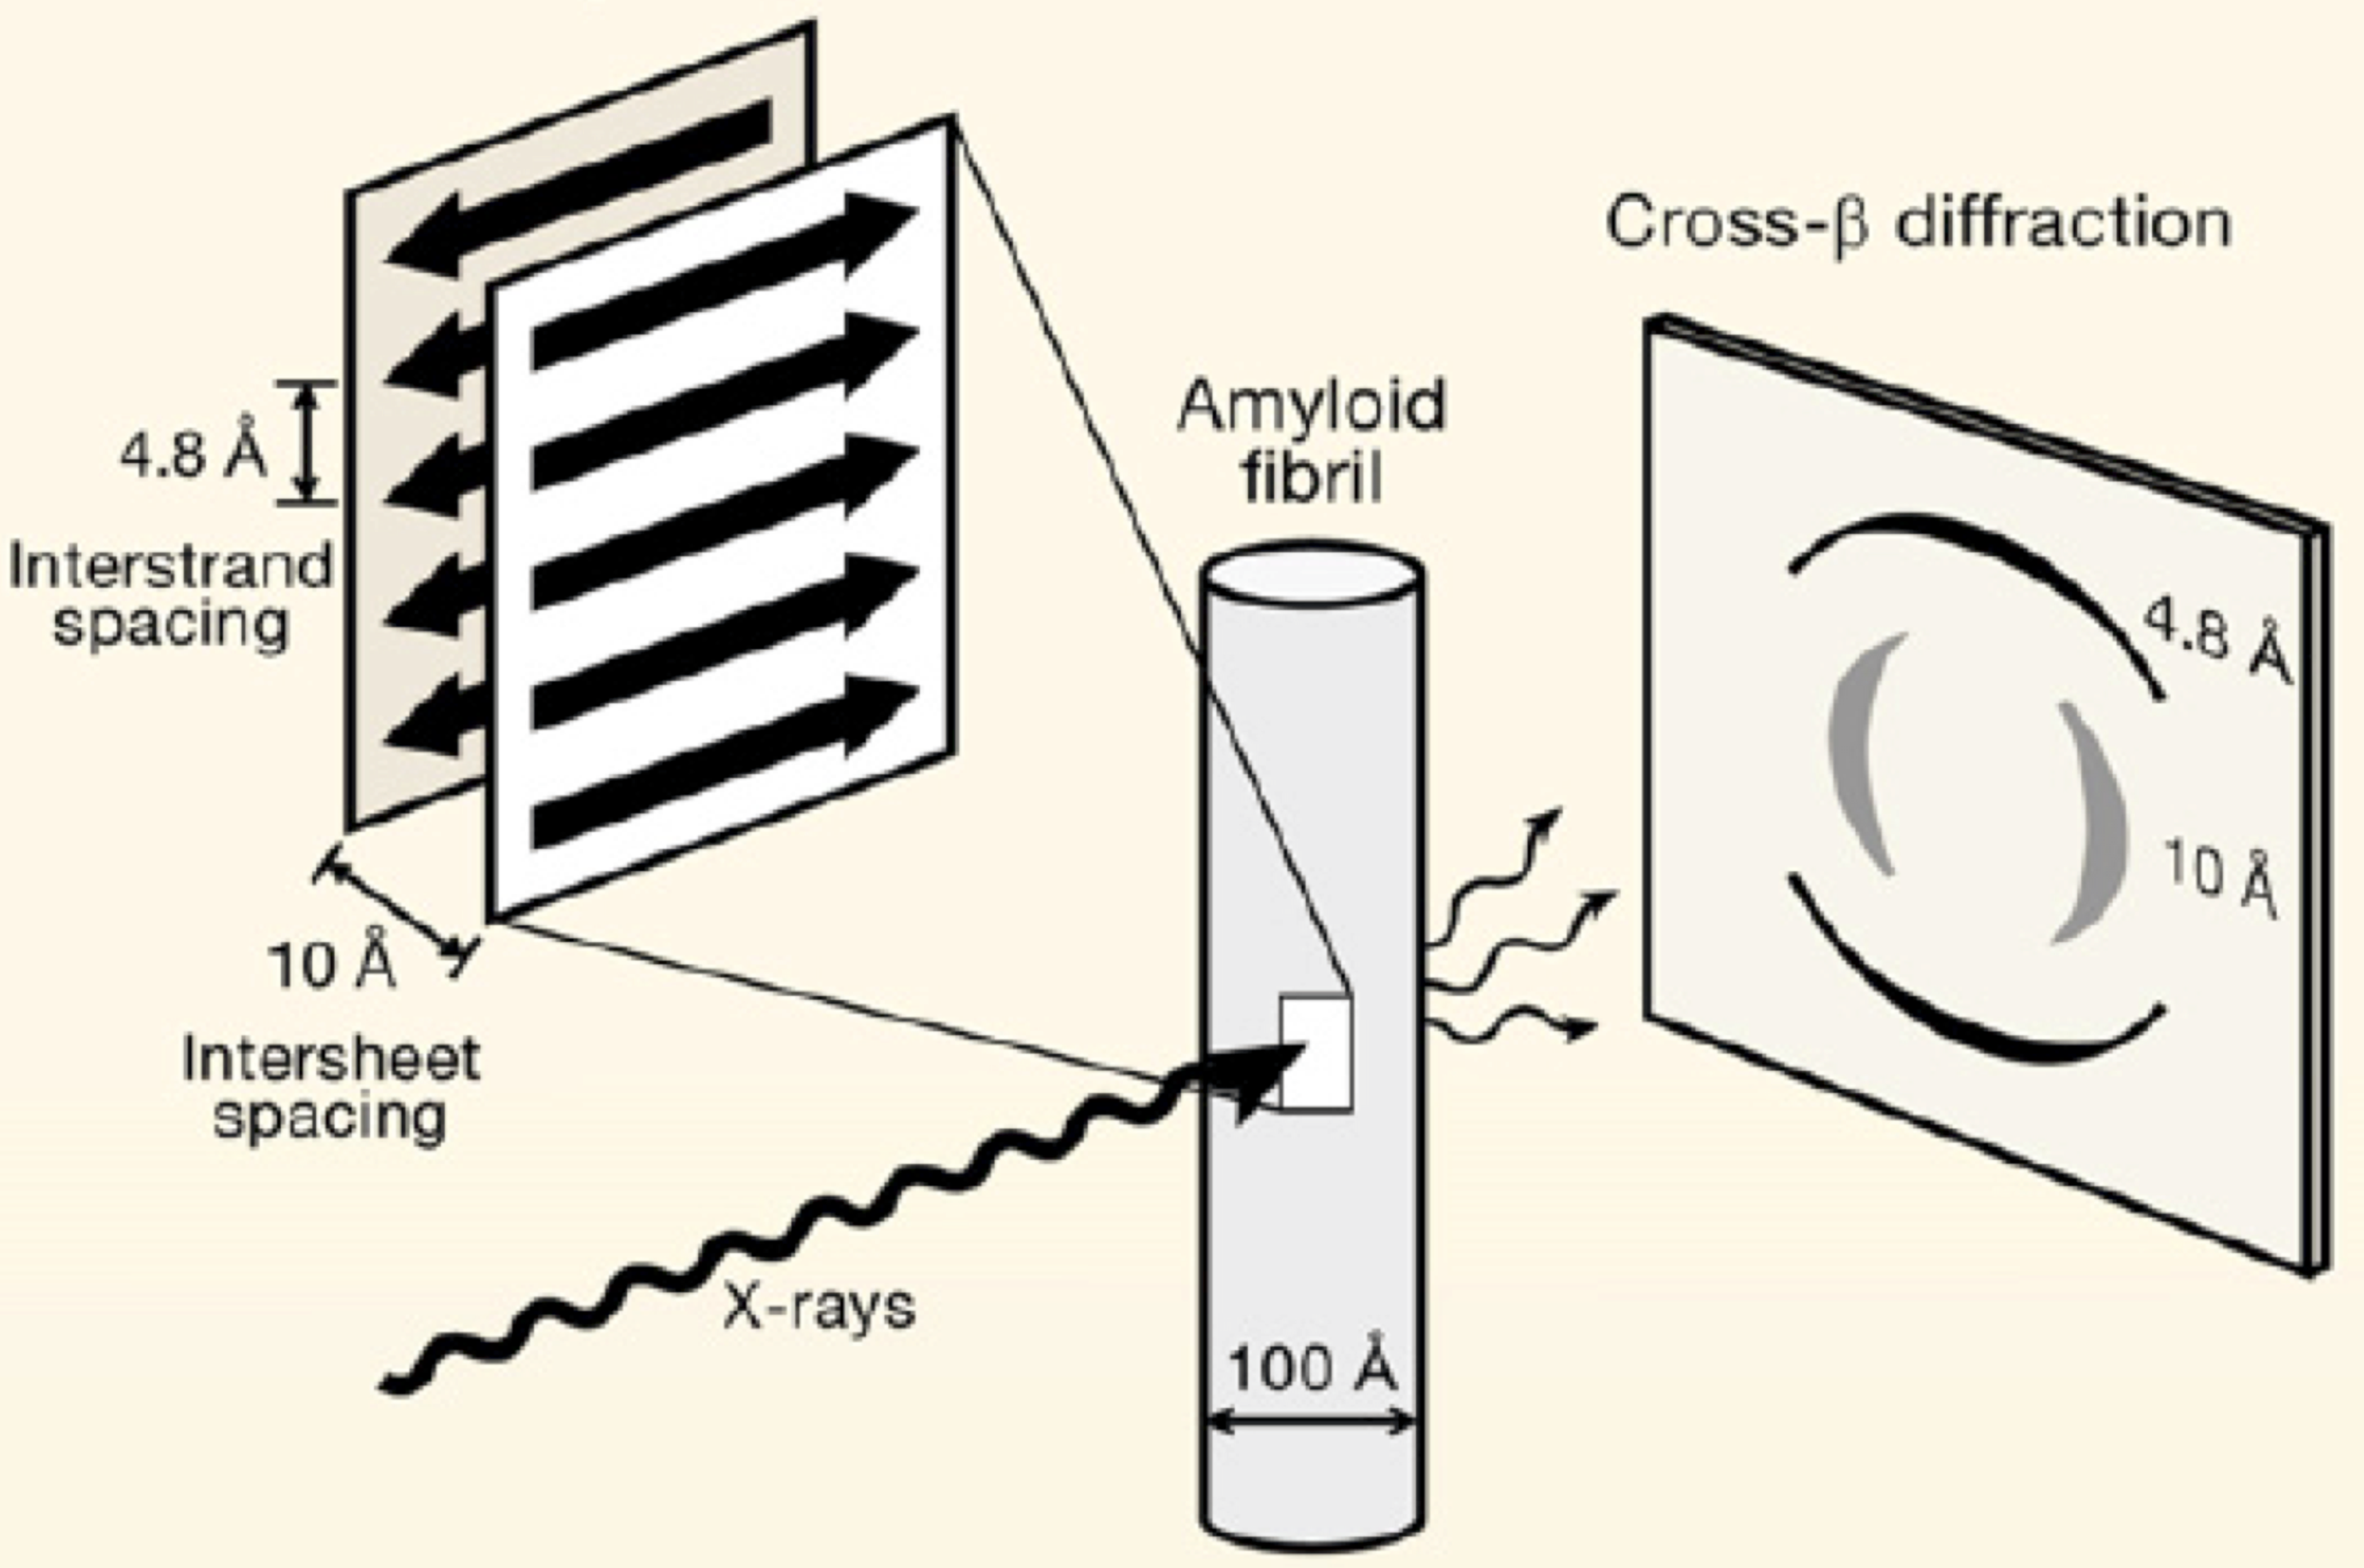
\includegraphics[width=6in]{figures/introduction/fibril_structure_diffraction.pdf}
  \caption[Characteristic cross-$\beta$ spacings from X-ray fibre diffraction studies of amyloid fibrils]{This is adapted from Eisenberg, 2012}
  \label{fig:fibril_diffraction}
\end{figure}

Despite having dramatically different sequences, amyloid fibrils formed from different polypeptides all adopt a similar morphology known as the \crossbs.  To date, independent measurements of fibrillar structure from different instruments have all confirmed the presence of \crossbs\ as the core structure of amyloid fibrils. \textbf{Initial structural studies, done using X-ray fiber diffraction, showed that fibril diffraction patterns are characterized by two major orthogonal reflections: meridional direction (along the fibril long axis) corresponding to a 4.8 \angstrom\ interpeptide separation, and perpendicular to the fiber axis (equatorial direction) has a  10 \angstrom\ intersheet spacing} (Figure~\ref{fig:fibril_diffraction}).  These defining measurements in fiber diffraction data have been adopted by biophysicists to be indicative of the presence of \crossbs, and hence, of amyloid fibrils. Furthermore, under the transmission electron microscope (TEM), fibrillar structures are visible as long, unbranched, and ribbon-like structures with diameters between 50 - 100 nms (Figure~\ref{fig:fibril_TEM_SSNMR}). 
% Other measurements? - MPL Mass per unit length?

% Although \crossb\ is widely known, due to the insolubility and inherent non-crystalline nature of amyloid fibrils, the molecular details of the fibril structure remained elusive until recent years. 
% The ubiquitous presence of a \crossbs\ supports that the organization of the peptidic backbone, common to all proteins, in to \bsheets\ is a major determinant of the fibrillar structure. 

\begin{figure}
  \centering
  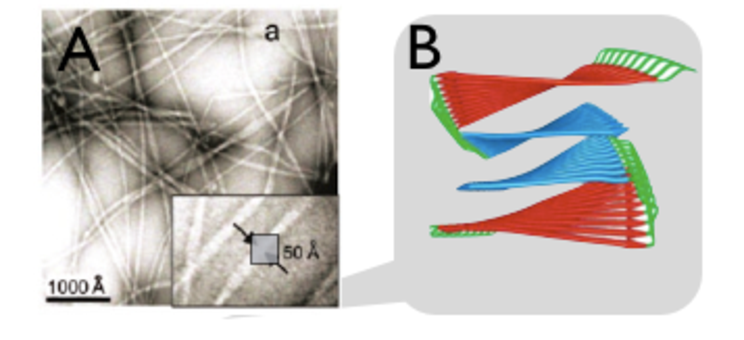
\includegraphics[width=6in]{figures/introduction/fibril_TEM_SSNMR.pdf}
  \caption[Characteristic cross-$\beta$ spacings from X-ray fibre diffraction studies of amyloid fibrils]{A Example EM images of oligomers.  Adapted from Bitan G. et al. 2003 and Walsh D. 1999 C TEM image of fibrils D SSNMR model proposed by Tycko et al.}
  \label{fig:fibril_TEM_SSNMR}
\end{figure}

\begin{figure}
  \centering
  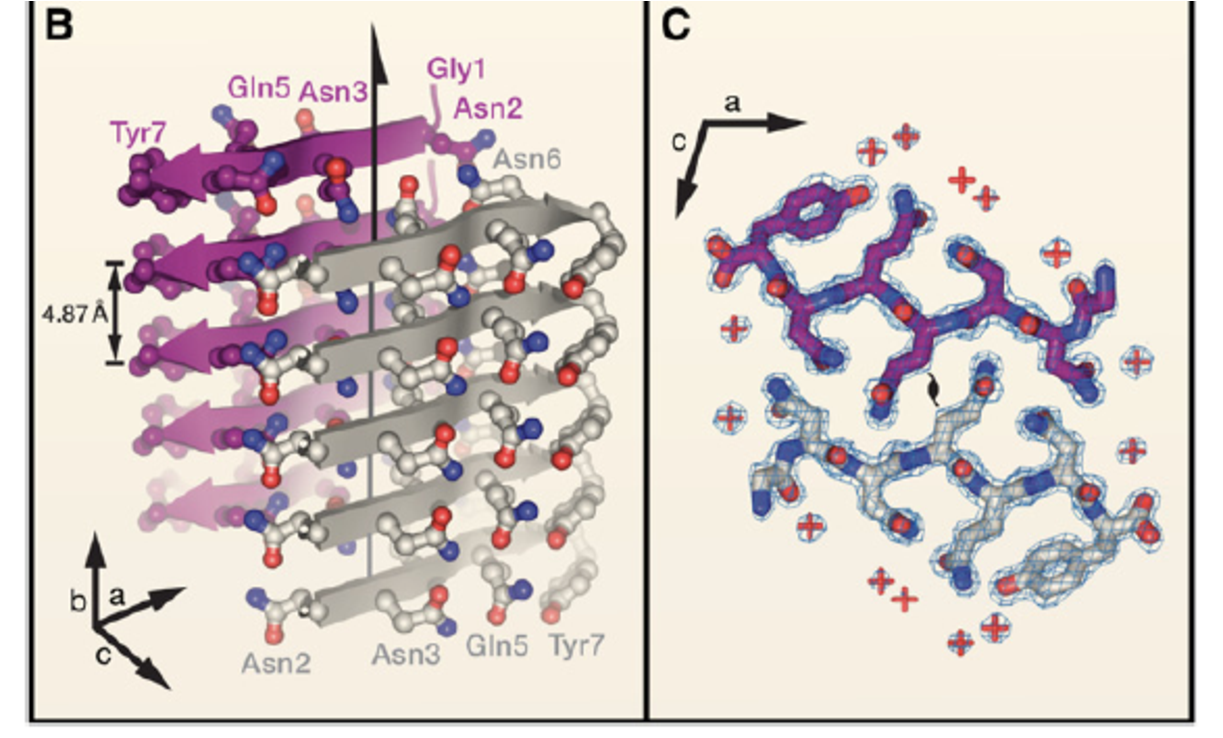
\includegraphics[width=6in]{figures/introduction/fibril_xray_model.pdf}
  \caption[Characteristic cross-$\beta$ spacings from X-ray fibre diffraction studies of amyloid fibrils]{This is adapted from Eisenberg, 2012}
  \label{fig:fibril_xray_model}
\end{figure}

% Describe the molecular structure of \abeta\ amyloid fibrils. Briefly mention the techniques that can be used to obtain structural information of amyloid fibrils. 

% SSNMR
Advances in solid-state NMR (SSNMR) and X-ray crystallography in the last decade have made major contributions to our knowledge of the molecular structure of amyloid fibrils. One of the early SSNMR model of an amyloid fibril was of the \abeta40\ peptide, a protein implicated in Alzheimer's Disease. The study by Petkova et. al.\cite{Petkova:2006gx} indicated that the \bsheet\ core of \abeta40\ involves residues 10-22 and 30-40, and is linked by a loop formed by residues 23-29. The core fibril unit was found to consist of a parallel in-register \bsheet, where each strand is a \bhairpin\ with peptide-peptide backbone hydrogen-bond running along the long axis of the fibril (Figure~\ref{fig:fibril_TEM_SSNMR}).

% X-ray structures
Aggregates formed from many different small peptide fragments of larger amyloidogenic peptides, which were amenable to single crystal X-ray diffraction analysis, produced crystal structures similar in structure to those resolved using SSNMR. These structures are composed of multiple layers of \bsheet\ with a dehydrated (``dry'') stacking interface (Figure~\ref{fig:fibril_xray_model}). Taken together, these recently proposed structures demonstrate that the core region is composed of two to four sheets that interact closely with each other. % I don't think I will talk about the twisting of the sheets too much. Should I mention twisting?

% Fibril polymorphism
Although all fibrils share the \crossbs, fibrils formed a peptide may exhibit polymorphism at the molecular level. Depending on the experimental conditions under which they are formed, fibrils may vary in the length of the $\beta$-strand involved, side chain orientation and inter-protofilament packing.\cite{Kodali:2007cz}  Fibril polymorphism may have important implications in amyloid diseases because, depending on which residues are exposed at the surface, different morphologies may have differing fibril toxicities. For example, in vitro, quiescently formed fibrils of A$\beta$(1-40) have been shown to be more toxic than agitated fibrils.\cite{Petkova:2005p4688}  A polymorphic structure introduced by a seed have been shown to be able to propagate in vitro.\cite{Paravastu:2006p4690} A recent study propagated a brain-derived fibril fragment in order to obtain structural information on fibrils that most closely resembles those formed in the AD brain.\cite{Paravastu:2009fi}
% http://onlinelibrary.wiley.com/doi/10.1111/j.1742-4658.2010.07888.x/abstract?systemMessage=Wiley+Online+Library+will+be+disrupted+on+15+December+from+10%3A00-12%3A00+GMT+%2805%3A00-07%3A00+EST%29+for+essential+maintenance

\subsection{Non-fibrillar oligomers}

Due to their structural disorder and transient nature, obtaining the molecular details of amyloid oligomers using traditional structural determination techniques have been impeded. However, advances in instrumentation and experimental techniques in recent years have begun to shed light on the structure of non-fibrillar oligomers. EM and AFM experiments have shown that transient, unstable particles may appear prior to the formation of fibrils. REFS
In particular, soluble \abeta\ protofibril assemblies that are annular, spherical, or curvilinear in shape have been reported in literature.\cite{Haass:2007db} Protofibrils may also bind to dyes Thioflavin T (ThT) and Congo Red (CR), suggesting the presence of substantial $\beta$-sheet content.\cite{Walsh:2007fu,Haass:2007db,Kodali:2007cz} 

Although these particles may be \bsheet-rich, they are morphologically distinct and are typically much smaller than fibrillar structures (Figure~\ref{fig:oligomers}).\cite{Walsh:2009p1235} However, it has been recently suggested that large non-fibrillar oligomers may contain fragments \crossb\ like in structure.\cite{Walsh:2010p4761,Stroud:2012dp,Chimon:2007du}  
\textbf{SOME ALSO DON'T BIND THT}

%A recent SSNMR study demonstrated that a late stage, neurotoxic Aβ40 spherical intermediate contained fibril-like β-sheet structure.16
% Should briefly read up on the book chapter by Pat Walsh and cite him

\begin{figure}
  \centering
  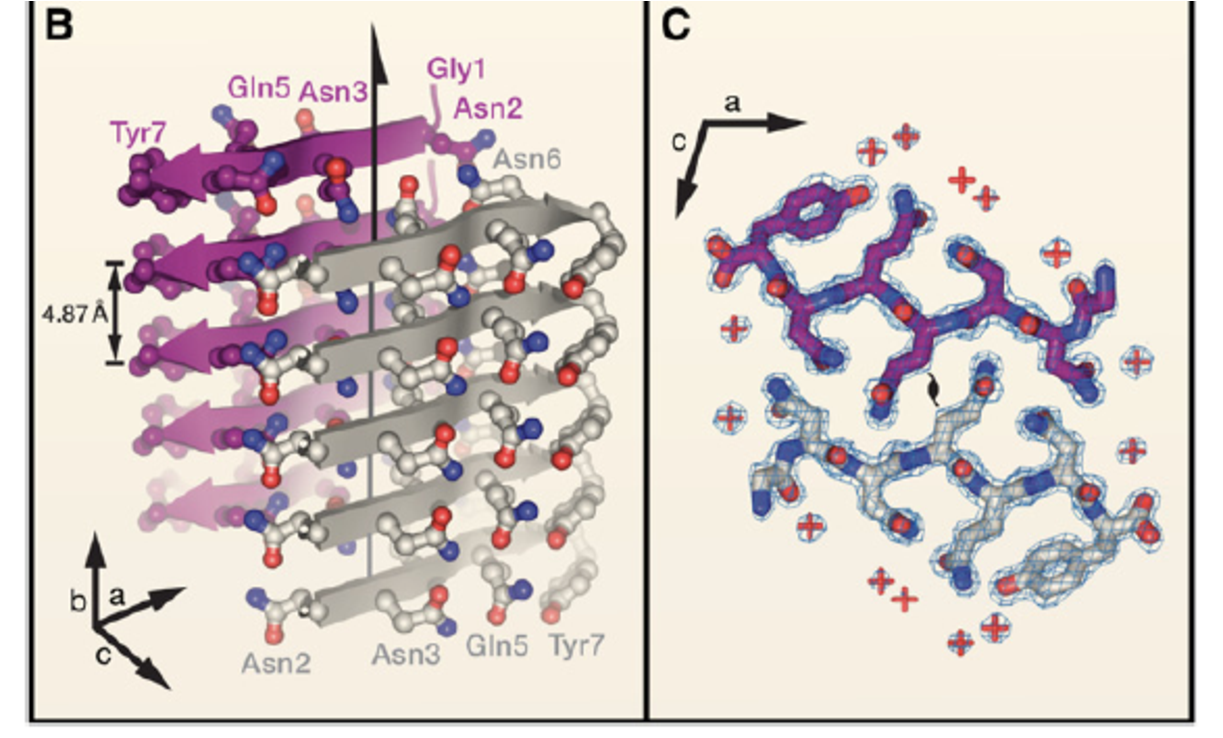
\includegraphics[width=6in]{figures/introduction/fibril_xray_model.pdf}
  \caption[Characteristic cross-$\beta$ spacings from X-ray fibre diffraction studies of amyloid fibrils]{This is adapted from Eisenberg, 2012}
  \label{fig:fibril_xray_model}
\end{figure}

\section{Amyloid involvement in diseases}

\begin{table}%\footnotesize
  \begin{center}
  \vspace{10pt}
  \caption{Summary of proteins which form amyloids}
  \label{tbl:amyloid_diseases}
    \begin{tabular}{| c | c | c | c |}
      \hline
      Peptide & Study & fibrils & oligomers  \\
      \hline
      \abeta\ & REFs & yes & yes \\
      alpha-synuclein & REFs & yes & yes \\
	  \hline
    \end{tabular}
  \end{center}
\end{table}

% Amyloid disorders other than AD -- In addition to AD, other neurodegenerative diseases have been shown to involve the presence of amyloid.  Parkinson's disease, Huntington's, Prion disorders (Mad cow).  These diseases and their pathology are reviewed elsewhere and are beyond the scope of the thesis. In this thesis we focus on AD.

% Outline some of the ideas / hypothesis about the link between amyloid and disease, but don't go into what people speculate or data on toxicity. It is related, but this is out of the scope of your thesis.

% Although not the focus of this thesis, understanding the mechanism of toxicity and elucidating the underlying toxic species will be important in the development of future drug candidates.

Because many disorders share the amyloid pathology, researchers initially hypothesized that fibrils found in amyloid plaques were toxic to cells. However, recent research has implicated soluble oligomers to be the most likely causative agent for toxicity in several neurodegenerative diseases: Alzheimer's, Parkinson's, Huntington's, and Prion-related diseases.\cite{Haass:2007db,Xue:2009da} % XXX The role of amyloid oligomers in the disease process is most intensively studied for AD. 

Pastor et al showed that short fragments of amyloidogenic peptides are toxic.\cite{XXX}

\textbf{SUMMARIZE SOME CELL CULTURE EXPERIMENTS HERE}
In AD, when oligomers are added to cells, the cells have been shown to demonstrate classic signs of neurotoxicity and even apoptosis.\cite{Cappai:2007bc,Lambert:1998ve,Walsh:2002p2566,Shankar:2008bg} Furthermore, it is believed that Aβ oligomers may initiate cell death and neuronal dysfunction.\cite{Cappai:2007bc}

The molecular mechanism of toxicity caused by amyloid oligomers is not understood. %Intensive research is currently being done to identify the toxic species in the amyloid aggregation pathway.  
Still an active area of research and the data is often very confusing. The central hypothesis of amyloid-induced toxicity is that soluble oligomers cause toxicity by binding to the lipid bilayer and perturbing the integrity of cellular membranes (perhaps by causing them to be permeable to ions).\cite{Martins:2008bz,Walsh:2007fu} Other mechanisms of toxicity induced by amyloid includes .. % REFs
\textbf{EXPAND ON THE VARIOUS HYPOTHESIS OF TOXICITY HERE. Find some biophysical support for this hypothesis -- there must be lots}
% One of the exam questions might be: Why is inositol toxic?

% I made it its own section because I currently don't support deeper than 3 levels of sections
% Also since I made the other one about amyloid toxicity as well, AD doesn't really fit there. But the transition to AD still works
\section{Alzheimer's Disease}

Alzheimer's Disease (AD) is a devastating neurodegenerative disease that is most common cause of dementia in persons of age 65 or older.  Upon examination, the post-mortem brains of AD patients show significant neuronal dystrophy.  Pathologically, AD is characterized by the presence of extracellular deposits of senile plaques and neurofibrillary tangles, which appear as lesions on stained neuronal tissue under light microscopy.(Figure~\ref{fig:AD_tissue_pathology})

% Pathological characterization
\begin{figure}
  \centering
  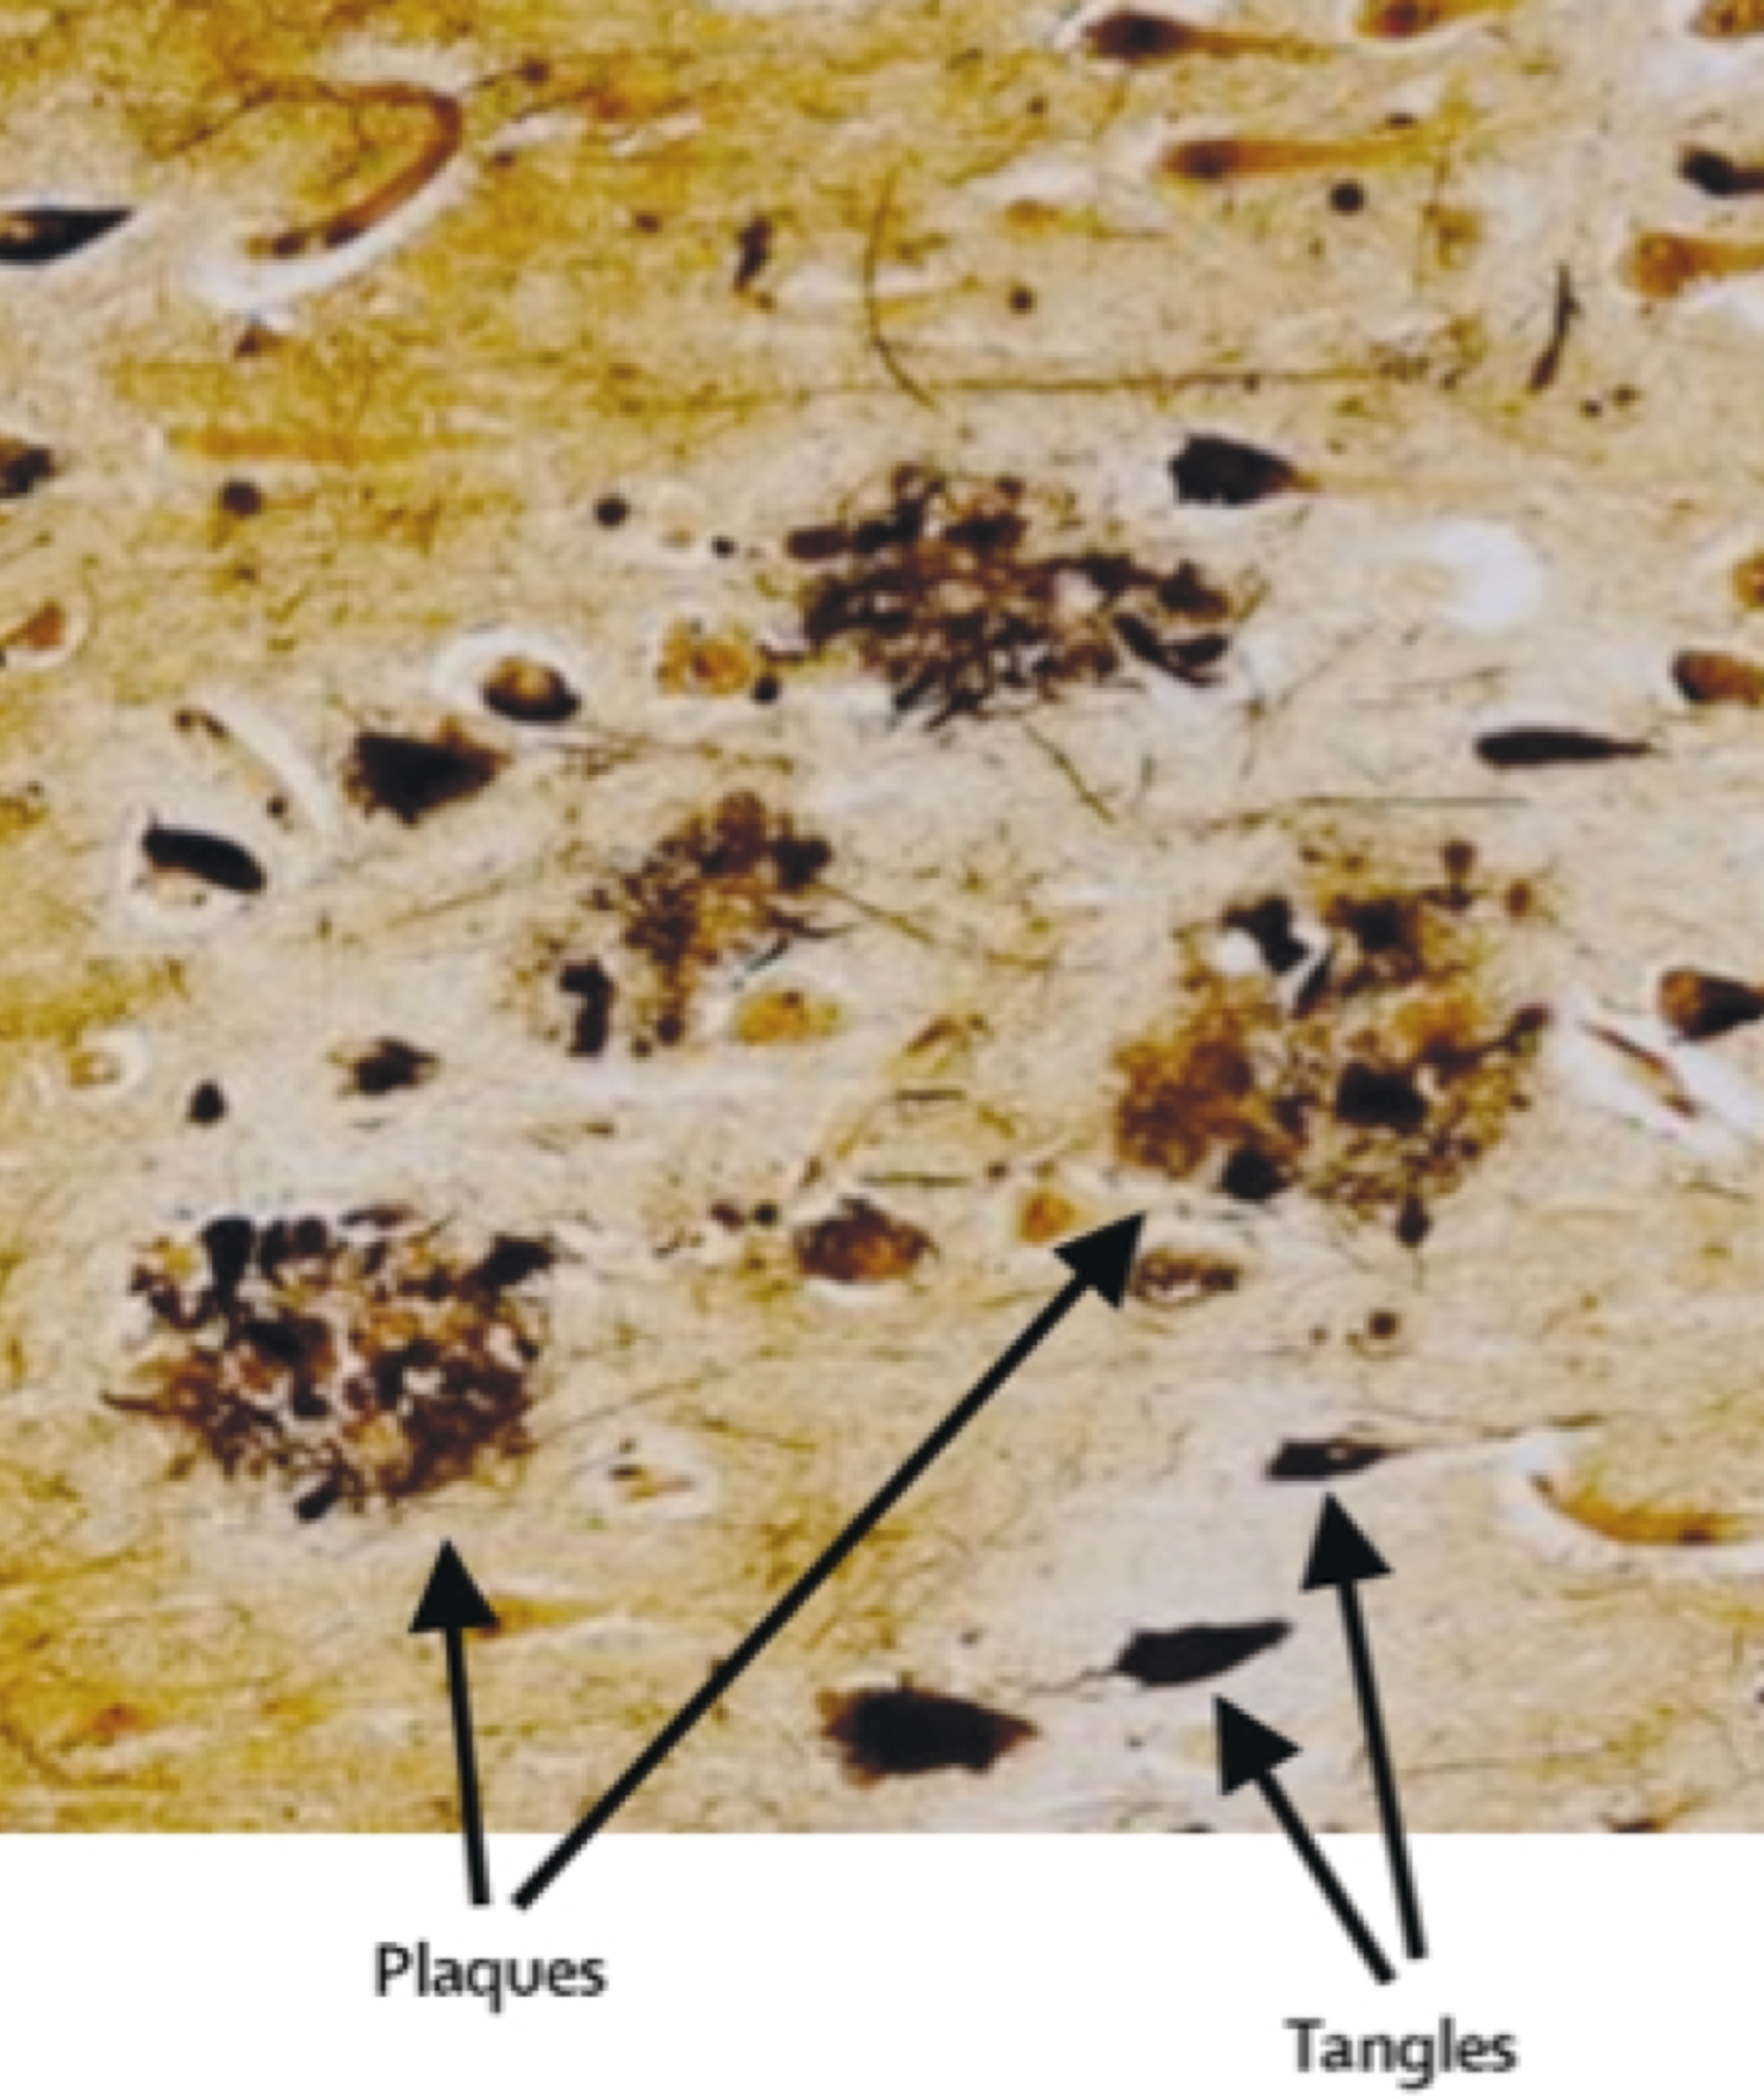
\includegraphics[width=3in]{figures/introduction/AD_tissue_pathology.pdf}
  \caption[Image of lesions formed by plaques and NFTs on brain tissue]{This is adapted from Blennow, 2006}
  \label{fig:AD_tissue_pathology}
\end{figure}

Although it has been more than one hundred years since Dr. Alois Alzheimer first presented the association between the presence of neuronal plaques and the clinical symptoms of presenile dementia characteristic of Alzheimer's disease (AD), the exact relationship between the two is still under much contention.  It was not until in the 1980s, the amyloid-$\beta$ protein or \abeta\ was identified as the largest component of these plaques.

\subsection{The \abeta\ peptide}

\begin{figure}
\centering
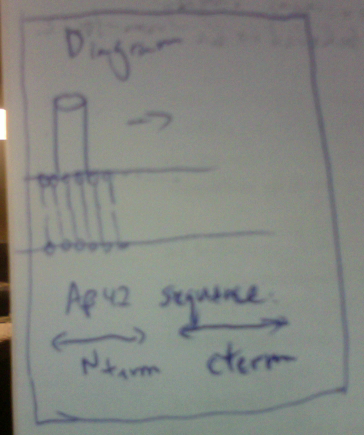
\includegraphics[width=3in]{figures/introduction/AD_abeta_app.png}
\caption[Abeta production]{Production of Abeta from APP}
\label{fig:AD_abeta_app}
\end{figure}

% Biochemistry of the Abeta peptide.
Monomeric \abeta\ is an approximately 4 kDa peptide produced by the intramembrane proteolytic cleavage of the larger amyloid-$\beta$ precursor protein (APP).  \abeta\ is produced constitutively as part of the normal cellular metabolism.\cite{Hardy:2002dh} APP is sequentially processed by the aspartyl proteases $\beta$-secretase and $\gamma$-secretase, where depending on the position of the cleavage by $\gamma$-secretase, a pool of \abeta peptides of lengths varying from 38 to 43 residues are produced. The peptides spanning residues 1-40 (\abetaforty) or 1-42 (\abetafortytwo) are predominantly found in AD-associated plaques. Neuritic plaques is composed of mainly \abetafortytwo, whereas \abetaforty\ is more commonly found in cerebral vascular plaques.

The ubiquitous presence of amyloid plaque deposits found in the brains of deceased dementia patients led to the formulation of the long-standing amyloid hypothesis, which posits that the amyloidogenesis of \abeta\ plays a key role in the initiation of AD.\cite{Hardy:2002dh} Support for the amyloid hypothesis comes from genetic evidence, particularly in those with trisomy 21 (occurring in Down's syndrome), the chromosome responsible for encoding APP. Furthermore, in familial AD, genetic mutations on the APP, which is responsible for developing early-onset AD were also found to have increased aggregation propensities in vitro. % REF -- the biochemistry of AD inside and out.

Multiple lines of evidence indicate that \abetafortytwo is likely to be the more deleterious form of \abeta. Genetic studies showed that mutations which cause early-onset AD also in turn increases the ratio of \abetafortytwo to \abetaforty.\cite{Hardy:1997tu} Moreover, in vitro, \abetafortytwo\ displays significantly higher propensity for aggregation than \abetaforty, despite differing by only two amino acids. In addition, \abetaforty\ and \abetafortytwo\ also have distinct aggregation pathways in vitro: \abetafortytwo is found to form a morphologically more diverse population of intermediate oligomers than \abetaforty.\cite{Bitan:2003ut} % What about mice studies?  LOOK AT DAVIS THESIS FOR MORE REFERENCES THERE IN SUPPORT OF ABETA42

% Tau protein - Keep discussion brief
Although both plaques and NFTs appear together, many studies have indicated that NFTs plays a secondary role to \abeta\ in the pathogenesis of AD.\cite{XXX} \textbf{EXPAND THIS PARAGRAPH} % More details on evidence which show that NFTs are not likely the causative species. Knock out mouse models ... mice do not develop AD, and instead develop tau pathologies  NFTs have also been shown to be affected by \abeta\ production.

% I think this detail about abeta aggregation in vivo is NICE TO KNOW but could be left out of the thesis.
% The concentration of Abeta in the CSF is in the low nanomolar range, but in vitro data shows that the critical concentration for aggregation is in the micromolar range. How does it then aggregate in the brain - mechanism of raising the effective concentration.

% In vitro models have been useful to screen compound libraries for inhibitors of agregation which may have therapeutic efficacy against AD.
A key question is what is causing AD? \abeta\ aggregates have been found to be present in a variety of morphologies in the brain. Although plaques are often visible in the dementia patients, the plaque load does not correlate with disease progression and severity, a puzzling aspect of AD.  Instead, synaptic loss correlated well with the concentration of soluble \abeta\ oligomers in the brain. \textbf{MORE DETAILS ON THE CURRENT ACCEPTED MECHANISM OF TOXICITY}

% Take a look at how Lemkul covers this section and transitions to it.
\section{Amyloid Inhibition by small molecules: A promising method of treatment for AD}
      
% Review of what is known about amyloid fibril ligand binding, specifically dyes.

% In this section, I will provide an overview of some of the challenges to overcome when developing a small molecule therapeutic for Alzheimer's disease.  Furthermore, using this information, I will motivate why inositol is an exciting avenue to explore.

% Briefly mention non-small molecule putative therapies which also acts via amyloid inhibition. The focus of this thesis will be on small-molecule amyloid inhibition.

% Amyloid inhibition as a treatment for Alzheimer's disease and related amyloid disorders. 
% Talk about how important it is to develop drugs for these amyloid disorders 
With the longevity of our population, AD is approaching epidemic proportions with no cure or preventative therapy available.\cite{Blennow:2006wd} In 2010, there are an estimated 36 million people in the world currently suffering from AD, and this number is projected to grow to 115 million people by the year 2050.\cite{alzreport:2012}  Furthermore, there are no drugs which may target the underlying disease: approved treatments today such as donepezil (a cholinesterase inhibitor), and memantine (a N-methyl-D-aspartate antagonist) only mitigates cognitive symptoms.
% \cite{Mangialasche, F. M., Solomon, A., Winblad, B., Mecocci, P., and Kivipelto, M. (2010) Alzheimer’s disease: clinical trials and drug devleopment’. Lancet Neurol. 9, 702�716.} \cite{(4) The 2012 PhRMA Report on Medicines in Development: Alzheimer’s disease. See www.phrma.org.} 

% PhRMA reports in their 2012 Medicines in Development Report for AD4 that there are currently 93 medicines in various stages of development, both small molecule and biologic. In general, all 93 compounds fall into one of the following therapeutic strategies: (1) agents targeting neurotransmission, (2) agents targeting Aβ production, (3) agents targeting Aβ aggregation, (4) agents targeting Aβ clearance, (5) agents increasing brain resistance to Aβ, (6) agents targeting tau protein, and (7) agents targeting neurotrophins and agents modulating synaptic plasticity and nerve growth.1−4 \cite{From the ACS neurochem's editorial letter}

% (1) Data from the Alzheimer’s association. See www.alz.org.
% (2) Data from Alzheimer’s foundation. See www.alzfdn.org.
% (3) Mangialasche, F. M., Solomon, A., Winblad, B., Mecocci, P., and Kivipelto, M. (2010) Alzheimer’s disease: clinical trials and drug devleopment’. Lancet Neurol. 9, 702−716. Special Issue: Alzheimer's Disease Published: November 21, 2012
% (4) The 2012 PhRMA Report on Medicines in Development: Alzheimer’s disease. See www.phrma.org. -- I should have a look at this report
% (5) Sadeghi-Nejad, N. (2012) The Lessons of failure: what we can learn from bapineuzumab’s blowup. Forbes (Pharma & Healthcare), August 7, 2012.
% (6) For information of the clinical trials with MK-8931, see www. merck.com.

Hence, it is imperative that efforts be made towards the development of therapeutics for AD.  The vast number of structural and biochemical studies on amyloid structure have been crucial for the development of potential therapeutics for treating the underlying disease.  A promising method of treatment of AD is by preventing amyloid aggregation, and decreasing amyloid production. Here is a paper summarizing current treatments for underlying disease\cite{Salomone:2012fh}

%Small molecules which prevent amyloid formation may be an effective method of treatment for amyloid disorders because of the potential to treat the underlying disease. 

A key pharmacological challenge of developing a drug for AD and other neurodegenerative diseases involves developing a small-molecule candidates, which also penetrate the blood-brain barrier (BBB) at sufficient concentrations for their therapeutic effects (ie. to inhibit amyloid formation). % Expand on this paragraph?
% Concentration at which the small molecule acts.  BBB penetration and bioavailability.

In recent years, in vitro screening has led to the discovery of a large number of small-molecules which were found to affect the amyloid aggregation pathway. Some inhibited amyloid fibrils, whereas others arrested or reduced non-fibrillar oligomer formation. Many of these small molecules are thought to act by directly binding to amyloidogenic peptides and aggregates. The main classes of molecules that have demonstrated promise as amyloid fibrillation inhibitors are reviewed in the sections below.
% Note that here I can take a cue from Justin Lemkul`'s recent review paper.

\begin{figure}
\centering
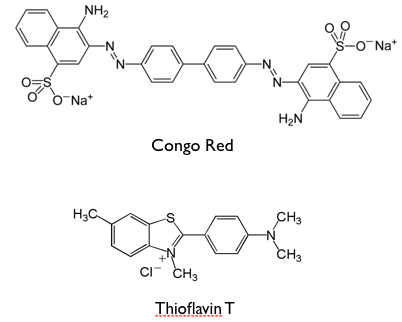
\includegraphics[width=3in]{figures/introduction/dyes.png}
\caption[Small molecule binders]{Amyloid binding dyes Congo Red and Thioflavin T}
\label{fig:amyloid_dyes}
\end{figure}

\subsection{Dye molecules}
% Molecular mechanism of binding of dye molecules. Thought to bind flat on on the surface grooves of amyloid fibrils where they interact with hydrophobic groups exposed at the surface. 
      % Doesn't explain why the dye molecules are also able to suppress fibril formation.
      % Can the birefringence be explained by these binding modes? -- this is out of the scope of my thesis.  Don't put this in my thesis but I should be able to coherently explain this during my defense.

Is it specific to Abeta amyloid inhibition? Or fibril structure or what? 
Any measured concentration of acitivity, IC/EC50, Kd of binding?
Biophysical data of binding and whether they've been adapted into a drug or were there attempts made to adapt into a drug.

Among the first molecules known to bind amyloid fibrils were dyes molecules used to identify their presence (Fig.~\ref{fig:amyloid_dyes}). Early histological detection of amyloid binding was done using congo red, where upon binding fibrils exhibit red-green birefringence. Congo red requires the use of polarized light microscopy, a laborious process, and the interpretation of the birefringence is often not reproducible.

% Thioflavin T (ThT) and Congo Red (CR)
Thioflavin-T (ThT) is a benzathiole fluorescent dye also used to detect the presence of amyloid fibrils in post-mortem brain tissue samples, and monitor fibril formation in vitro. ThT exhibits a dramatic shift in the excitation spectrum maximum and an emission enhancement upon binding to fibrils, making it a sensitive and efficient report for the presence of amyloid fibrils.  ThT is soluble in water and have \KD\ in the low \micromolar\ range.  ThT also binds uniformly across fibrils prepared from synthetic and biological sources.
REF

Due to the ubiquitous use of ThT as a amyloid fibril probe, fibril binding by ThT is well-characterized.  ThT doesn't always bind, and its binding depends on the physiochemical properties of the amyloid fibril.  ThT has been modified to bind to different fibrils.\cite{XXX}

% which led to the adoption of ThT dye binding as not only an indication of the presence of fibrils, but also as an indication of the presence of the \crossbs.
Dye molecules have been used as scaffolds to develop new imaging agents (for example, Pittsburgh compound B), and new molecules to stain amyloid fibrils for different sequences. 

% Methylene Blue is a histological dye molecule shown to promote the fibrillation of Abeta.
% It is coming back in clinical trials -- shown I review that?
% http://www.ncbi.nlm.nih.gov/pubmed/17595112

% How does it bind? And what causes the fluorescence when it binds?
The studies by Naiki et al. and LeVine et al demonstrated the link between ThT dye binding and the presence of \crossbs\ of fibrils. Binding in hydrophobic groups on fibril surfaces and is characterized by hydrophobic interactions ...
Crystallography studies have shown possible binding modes of dye and dye-based molecules with fibril fragments.\cite{XXX}

Orange-G molecules were recently crystallized with amyloid-like peptide segments from Tau and Abeta.  In the crystal structures, orange-G 

Charge was shown to modulate the binding mode: charged molecules can binding between two sheets by making polar and electrostatic interactions.
% http://www.plosbiology.org/article/info%3Adoi%2F10.1371%2Fjournal.pbio.1001080

At a particular concentration, these dye molecules were also found to impede fibril formation.\cite{XXX}

ThT binds hydrophobic pockets in globular proteins: It has been shown to bind to a hydrophobic pocket of human serum albumin with comparable affinity to many drug-like molecules.\cite{Groenning:2007p3436,Groenning:2007eo}

% Furthermore ThT fluorescence is only observed from those molecules that have bound to the fibrils.  
% ThT exhibits a shift in the excitation spectrum maximum, from 385 nm to 450 nm, and the emission maximum, from 445 nm to 482 nm

% This is from \cite{Wu:2011fd} which briefly summarizes why ThT binding gives rise to the excitation spectrum.
% These phenomena stem from two effects of binding.
% Firstly, steric and electronic stabilization (via charge trans- fer) of the ground-state charge distribution (7,8); and 2), restriction in the rotation of the aromatic rings of the dye (see Fig. 1 A) in its electronically excited state (9,10).

% Being \bsheet-rich does not imply that these dye molecules would bind. Also can affect fibril formation.

\begin{figure}
\centering
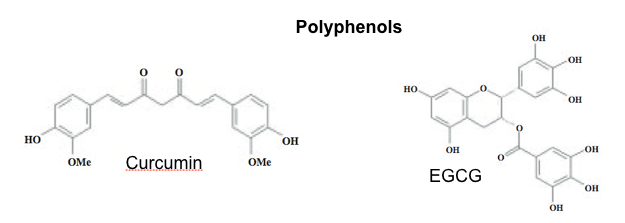
\includegraphics[width=6in]{figures/introduction/polyphenols.png}
\caption[Small molecule binders]{Polyphenols}
\label{fig:polyphenols}
\end{figure}

Simulation studies have shown that ThT / CR bind at surfaces of fibrils, adopting two main modes of binding: XXX.\cite{XXX I'm thinking of the Chun Wu study from 2007, were there more?}

\begin{table}%\footnotesize
  \begin{center}
  \vspace{10pt}
  \caption{Summary of small molecules known to affect amyloid formation}
  \label{tbl:inhibitors}
    \begin{tabular}{| c | c | c |}
      \hline
      Molecule & Study & Mechanism of action \\
      \hline
      ThT & REFs & Binding to fibrils \\
      EGCG & REFs & Binding to toxic oligomers \\
	  \hline
    \end{tabular}
  \end{center}
\end{table}

\subsection{Polyphenols}
% Where are they found? Plants, animals, in food. What are they used for in nature?
% Chemical features of polyphenols? Properties? Soluble?
% What is known about their molecular mechanism?
Polyphenols is a class of molecules found both naturally in plants. They can also be made synthetically. Recently experimental evidence suggests that three such molecules X, Y, Z modulate \abeta\ aggregation, and hence may be developed into therapeutics for Alzheimer's Disease and related neurodegenerative diseases.  In this section, the discussion will be focused on these compounds and their role in fibril inhibition.

Most common subgroup of phenolic compounds are flavonoids, known for their anti-oxidant properties, were shown to modulate amyloid formation (Fig.~\ref{fig:polyphenols}). They have a high EC50 for the inhibition of fibrils.   (−)-epigallocatechin-3-gallate EGCG is the major polyphenolic component of green tea and  A variety of experimental in vitro cell culture paradigms have shown micromolar concentrations of EGCG to be protective against Ab-induced cell death [Bastianetto et al., 2006; Kim et al., 2007; Levites et al., 2003].

Only begun to explore their molecular mechanism of binding [Do they have similar mechanism of action? What are their advantage and disadvantages as a therapeutic for AD?]

% curcumin
% New papers :
% http://pubs.acs.org/doi/abs/10.1021/cn3001203
% morin

\subsection{Non-steroidal Anti-inflammatory compounds (NSAIDs)}

% Naproxen and ibuprofen
% From \cite{Takeda:2010gx,Raman:2009jn}
CUT THIS SECTION DOWN

% I don't think I need to include a whole paragraph summarizing ibuprofen.  It's the same story as inositol.
One of the potential candidates is a nonsteroidal anti-inflammatory drug (NSAID) naproxen and ibuprofen (\ref{fig:nsaids}).\cite{XXX} Epidemi- ological studies have shown that chronic prophylactic intake of naproxen moderately reduces the risk of AD.12,13 Furthermore, reexamination of the results of large-scale clinical trials suggests that under certain conditions naproxen can reduce the AD risk by 67\%.11

Biomedical studies suggest that treatment with ibuprofen reduces the amount of Ab deposits and alleviates memory deficits in mice models (17,18). Ibuprofen intake also correlates with a decrease in the amount of Ab oligomers in mice brain tissues (18). A prophylactic long-term use of ibuprofen appears to reduce the risk of AD (19), but the effectiveness of this drug against preexisting AD cases is unclear (20). 

Several recent experimental studies have investigated the molecular aspects of interactions between Ab and ibuprofen. Binding of ibuprofen to Ab fibrils has been demonstrated when the ligand/peptide stoichiometric ratio approximates or exceeds 1 (21,22). 

Experimental in vitro studies have shown that ibuprofen reduces accumulation of Ab fibrils by apparently interfering with fibril elongation (23). Furthermore, ibuprofen demon- strates an ability to at least partially dissociate preformed Ab fibrils (21,23).

\begin{figure}
\centering
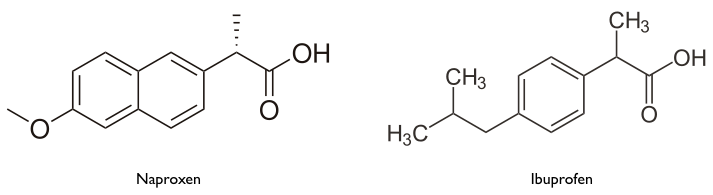
\includegraphics[width=4in]{figures/introduction/nsaids.png}
\caption[NSAIDs]{NSAIDs}
\label{fig:nsaids}
\end{figure}

\subsection{Inositol}
% Here we will review the physiological role of inositol in nature, and introduce inositol as a potential therapeutic for amyloid disorders. Here, use the physiological role of myo-inositol as a lead to transition into its role in amyloid inhibition.
\begin{figure}
	\centering
	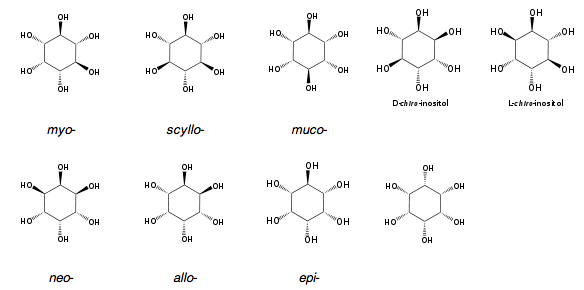
\includegraphics[width=6in]{figures/introduction/inositol.png}
	\caption[Inositol]{Inositol stereoisomers}
	\label{fig:inositols}
\end{figure}

Inositol with the molecular formula of \ce{C_6H_12O_6}, is a simple polyol with nine naturally occurring stereoisomers. Out of these nine isomers, seven are optically inactive, and the remaining two (L- and D-chiro-inositol) are chiral enantiomers.(Figure~\ref{fig:inositols}) Myo-inositol, the most abundant isomer, is ubiquitous in all eukaryotes and is a physiologically important osmolyte.  Furthermore, myo- is a precursor for inositol lipid synthesis: It is a constituent of phosphatidylinositol, an important phospholipid in membranes and second messenger systems. Once phosphorylated, myo-inositol phosphatides act as second messengers in intracellular signal transduction pathways.\cite{Fisher:2002tk} Some specific pathways which involves inositol are XXX ... YYY.\cite{Michell:2008dh}

Inositol is found in high concentrations in tissues of the human central nervous system (CNS): myo- And scyllo-inositol have approximate concentrations of 5 and 0.1-0.5 mM in the CNS, respectively.\cite{Fisher:2002tk} Accordingly, inositols also function as osmolytes in the CNS, where alterations in their concentrations are known to be associated with neuropathological conditions.\cite{Michaelis:1993gf, Fisher:2002tk}

% Role of inositol in amyloid inhibition. Here, include the background on how inositol was discovered as an \abeta\ amyloid fibril inhibitor. Should try to make it into a little story of how inositol was discovered. 
In recent years, scyllo-inositol have been identified as a promising therapeutic candidate for the treatment of Alzheimer's Disease. \textbf{ADD MORE DETAILS ON HOW IT WAS DISCOVERED.  IT MUST SOMEWHERE IN JOANNES PAPERS} 
% MAKE A LIST OF HER PAPERS AND SUMMARIZE WHAT EACH PAPER SAYS.  MOVE CITATION WHEN NEEDED.
Moreover, inositol exhibits stereochemistry-specific effects on \abeta\  fibril inhibition and cytotoxicity: \cite{McLaurin:2000bq} Scyllo-, myo-, and epi-, but not chiro-inositol, have been shown to inhibit \abeta42 fibril assembly, stabilize an oligomeric complex of \abeta42, and attenuate \abeta-oligomer-induced neurotoxicity in vitro. 

An important therapeutic advantage of scyllo-inositol is its ability to readily crosses the bloodbrain barrier (BBB) (both actively and passively transported).  Because it is not enzymatically broken down in the gut, it can be developed into an orally administered drug. % Inositol is synthesized inside the body ... or can be obtained via nutrition?
In vivo studies with a transgenic mouse model of AD demonstrated that alleviation of symptoms after inositol treatment was correlated with a decrease in the levels of soluble \abeta\ oligomers, suggesting that the beneficial effects of scyllo-inositol may be attributed to the inhibition and/or disaggregation of high-order \abeta\ oligomers.\cite{McLaurin:2006eb}
Presently, scyllo-inositol has completed both phase I and II of human clinical trials.  Inositol was found to be non-toxic to healthy individuals at concentrations effective for amyloid inhibition. Taken together, these results suggest that scyllo-inositol, and its derivatives, are a potential therapy for AD with the ability to change the course of the disease.\cite{Nitz:2008jl,Sun:2008ko}  A central focus of this thesis is on elucidating the molecular mechanism of inositol binding to amyloidogenic proteins and peptides (in particular A$\beta$).
\textbf{ADD MORE DATA ON CLINICAL TRIALS}
% Include some data on human clinical trials (?) -- II was negative ... how to say it ? Should read phase II paper.

% Distribute this section to the above section
\subsection{Mechanism of action of small-molecule aggregation modulators}
% Here I can refer / discussion how small molecule binding might be different from classical binding (However, I feel like discussions might not be appropriate in this section!)

% Mechanism of action.
Some small molecules inhibit fibril formation, where as others may prevent oligomerization, but not fibrillation. A high concentration is often required to observe activity (micromolar to millimolar), which suggests that they may be non-specific, and have much weaker binding affinities compared to classical inhibitors of enzymes, which typically binds with nanomolar Kds. EGCG, one such polyphenol, is known to have the lowest IC50.  These \smi\ which act on species often without a well-defined morphology such as those of globular proteins, do not fit entirely within the classical enzyme inhibition model. They are able to be active at much lower affinities, and do not bind in one specific binding pocket.  Although the concentration of their activity is high compared with classical inhibitors,  they are still below co-solvent and osmlarity levels, which suggests these \smi\ may affect aggregation by directly binding to amyloidogenic peptides and / or aggregates.

What is the evidence for direct binding? NMR studies indicate direct binding activity for several small molecules.\cite{XXX EGCG paper nature 2007}.  EGCG was found to directly bind to alpha-s and Abeta.

A single small molecule may inhibit the fibril formation of different peptides.

%\subsection{Structure-activity relationship of small-molecule inhibitors}
% Describe and discuss observed commonalities between small molecules which appear to affect amyloid aggregation.
Small molecule inhibitors share common chemical features and groups.  They are typically planar in geometry, have many aromatic rings, and polar functional groups (hydroxyl groups) around the edge of these aromatic rings.\cite{Stempler:2011dy,Shoval:2007p3547,Porat:2006fn,Lemkul:2012da}

% This section provides a nice lead in to the methods section
\section{Rational drug design}

\begin{figure}
	\centering
	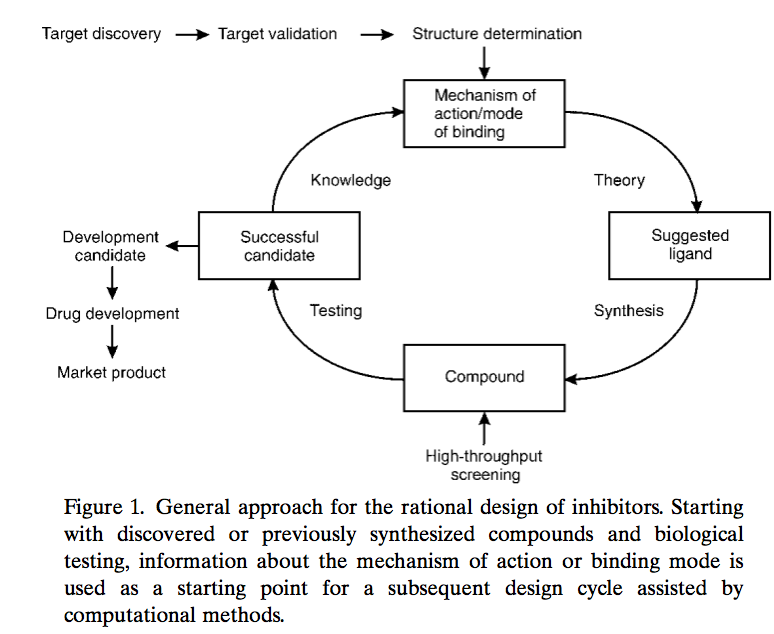
\includegraphics[width=6in]{figures/introduction/drug_discovery_flowchart.png}
	\caption[Rational drug design]{Diagram explaining rational drug design adapted from\cite{Gohlke:2002in}}
	\label{fig:rational_drug_design}
\end{figure}

Below is a summary of an excerpt from Tom's thesis on structure-based drug discovery.

Design of antibiotics example: 

1) Target determination (biochemical)

2) Structural determination (Xray, NMR, or homology); active site identified; Here would be useful to get the holo structure of the protein

3) Screen for inhibitors against a chemical library or in silico docking.

(see Figure~\ref{fig:rational_drug_design})

\section{Protein-ligand binding}

% Here is the description of target - ligand binding mechanisms in the "classical pharmacological case"
% I don't have to describe this in detail, but I think a section should set the reader up for understanding binding to amyloid ... and how that compares and differs from the classical pharmacological perspective of targeting a protein such as an enzyme ("What people normally think of").

% [Note that I have yet to really find any study with measured Kd or IC50 for amyloid inhibiiton]

% Regis -- Binding equilibria include both modes and binding constants

These references will help me in part flesh this section out.\cite{Lu:2010jh,Kortagere:2010fc,Nunez:2012il,Copeland:2011dl,Prinz:2008kr,Sikazwe:2012gu,Copeland:2006bb}

% Pharmcology metrics to assess drug efficacy (if a drug is “working”)

% \subsection{Enzyme-Inhibitor Binding and Kinetic model}
% Take a look at a biochemistry textbook

Kinetics and equilibria metrics used to characterize a lead compound. The in vitro interaction between a receptor and ligand is quantitatively assessed by equilibrium measures of binding affinity, such as IC50, the equilibrium dissociation constant or the Gibbs free energy of binding. These quantities are related to each other.
Go on to discuss each of these in a little more detail:
introduce terms such as EC50 or IC50

% Here would be a section explaining the desirable traits of a drug for AD

Binding kinetics is concerned with the rate constant of ligand association ($k_{on}$) and ligand dissociation ($k_{off}$). The ratio of the dissociation to the association rate constants establishes the equilibrium dissociation metric of the ligand (Kd = koff/kon), which determines the fraction of receptor occupancy at specific ligand concentrations; 

% K , k and k are intrinsic to the target
% There are two general binding mechanisms for a target–drug pair -- not really you can get more complex if you like
In mechanism 1, the receptor (R) and ligand (L) combine to form a binary complex RL with association/dissociation rate con- stants k1 (kon) and k2 (koff), respectively (Eqn (1))

In mechanism 2, the ligand encounters the receptor (R) in a conformational state that is suboptimally complementary to the ligand for binding. Subsequent to the initial encounter (RL), the receptor undergoes a conformational change to a more committed state (R*) where the new binary complex (R * L) competent binding affinity than RL (Eqn (2)).
Two equilibrium dissociation constants are required to describe this so-called ‘induced fit’ mechanism -- do I really care about this?

% Hence, the value of koff for mechanism 2 is not defined by a single microscopic rate constant. Instead, koff entails an array of diverse rate constants associated with both RL and R * L, such that koff = k2k4/(k2 + k3 + k4). In most instances, it is the reverse isomerization rate constant k4 that is rate limiting with respect to R * L dissociation. This isomerization step adds significant potential for a more enduring partnership between the target and the ligand (Table 1). In fact, most ligands with resilient kon and koff rates are dictated by mechanism 2, in which a temporal isomerization (e.g. tautomerization) of the target (and/or ligand) to a novel state is most suitable for target–drug binding to occur [8,9].

% These are important to know -- but I don't think I need to include their descriptions in the thesis

% At this point, it is important to highlight two common scenarios where a target and its ligand physically encounter each other in solution. The first is termed the ‘closed system’, where the total receptor and ligand concentrations are constant over time. In this scenario, the only change in concentration that takes place over time is the concentration of free and bound species as the system approaches equilibrium. Thereafter, the measurements of equilibrium dissociation constants are performed [5]. In this case, the target–drug complex lifetime is approximated by the equilibrium dissociation constant [1].

% The second scenario is the open system, which is more relevant to physiological conditions. Here the receptor is typically kept at a fixed concentration whereas the ligand concentration is allowed to vary, mirroring factors such as metabolic clearance or diffusion through cellular compartments. Thus, the open system is characterized by continuous changes in the flux of ligand that is available for encounter with the receptor. Because the concentration of the ligand continuously changes in an open system, equilibrium measurements are not feasible.

% The structure–activity relationship (SAR) is the relationship between the chemical or 3D structure of a molecule and its biological activity. 

% IC50 -- This quantitative measure indicates how much of a particular drug or other substance (inhibitor) is needed to inhibit a given biological process (or component of a process, i.e. an enzyme, cell, cell receptor or microorganism) by half.

% EC50 -- The term half maximal effective concentration (EC50) refers to the concentration of a drug, antibody or toxicant which induces a response halfway between the baseline and maximum after some specified exposure time.[1] It is commonly used as a measure of drug's potency.
% Ref: wikipedia

% Pharmacology in vivo - idea that drug residence times important for activity

% This is a potentially relevant side idea which came out of my readings that I can weave into the conclusion. Copeland et. al. argues that residence time is more indicative of drug efficacy in vivo … (but I fail to grasp how a drug can have the same Kd but different dissociation rates.  So for example if a drug comes off and goes on fairly fast, doesn’t that also imply that the drug is also bound for a relatively short amount of time?  Or perhaps my understanding of binding rates is flawed.)  copeland says that measuring the residence time is important because it is independent of whether the protein-ligand binding studies are done in a closed (like in vitro systems) or open (where the target and ligand concentrations are in dynamic flux -- and so Kd may not be an appropriate measure of efficacy). \cite{Tummino:2008bd,Copeland:2011dl,Copeland:2006bb}

% [More for the conclusions] Here I can link this to MD .. in MD we can calculate the drug residence times as well to get an idea of how long the receptor-ligand complex may last.  It is likely that this may be an important property for amyloid inhibition as well … what should be the rest of this logic? I think the connection for me here ends at the fact that we can also estimate residence lifetimes from simulation data: Modelling and simulations is a promising approach for drug design because of the wealth of data available from just a single atomistic simulation trajectory. For example, one can easily determine X, Y, Z … and in vivo drug residence lifetime is one such property that is useful to predict


\subsection{Binding equilibria}

The dissociation constant, $K_d$, is a measure of the affinity of a ligand for its binding site on the host protein. Pharmacologically, it can be interpreted as the concentration at which 50\% of the drug is bound to the protein. In experimental studies, $K_d$ is used as a measurement of drug potency and is used to quantitatively screen for potential drug candidates.  A low $K_d$ indicates that the ligand is tightly bound (high affinity binding) to its binding site on the protein.  Enzyme and its putative ligand typically bind specifically high affinity binding.  Rational drug design is often applied to optimize ligand binding specificity in an effort to increase the efficacy of the putative drug, and decrease adverse side effects (toxicity) in the human body.

The chemical equilibrium for the binding reaction is given by,

    \begin{equation}
      \left[ Protein\cdot Inositol \right] 
      \rightleftharpoons 
      \left[ Protein \right]+\left[ Inositol \right]
    \end{equation}
  
    % \2 Absolute binding free energy
    % \2 Relative binding free energy
    
The binding free energy of a ligand to a protein is directly related to its dissociation constant, $K_d$, the equilibrium constant of the above reaction

    % Kd equation
    
     \begin{equation}
        K_{d} = f_{ub}\frac{\left[ Protein \right]\left[ Inositol \right]}{\left[Protein \cdot Inositol\right]},
     \end{equation}
     
     % Free energy equation
     \begin{equation}
        K_{d} = e^{\frac{-\Delta G}{RT}}
     \end{equation}

     \begin{equation}
        \Delta G = -RT\ln K_d
     \end{equation}
     
% Add equation converting binding constant to gibbs free energies.
% Nov 23, 2012: Might be nice to have here but do I really want to defend this?
% \1 Experimental techniques for estimating $K_d$
% \2 What experimental techniques are used to estimate binding affinity? (May need to study up on this)
% \2 Isothermal titration calorimetry (ITC) is a technique which can be used to measure energetics of ligand binding to peptides.

% Link to the next section on protein-carbohydrate interactions 
Inhibitors of enzymes bind with affinities typically in the nanomolar to micromolar range.  For example, XXX (where can I find some examples?) However, a class of protein-ligand binding interaction, where a high \KD\ (weak affinity binding) is found are protein that bind carbohydrates is one such class of proteins, where weak interactions (low affinities in the millimolar range) between carbohydrates enable their function.

\subsection{Multivalency in binding}
% Definition and description of binding avidity
Above describes the quantitative measure for a ligand binding to a single specific binding site on its target.  However, there are cases where a ligand can binding in several binding sites at once, where the a single interaction of the ligand with the receptor site is fairly weak, but the ligand achieves its specificity of binding via forming multiple interactions.  In this case, we talk about a binding avidity.

\subsection{Intermolecular forces involved in binding}

% HBs involved in Binding.
% - What are the energetic contribution of these hydrogen bonds? (How are they measured?)
% osmolytes
% solvent - solvent interactions
% O-H ... O-H

% There lots of different forces; so am I present them as the ones modelled in simulation?
% then I need to mention computer simulation earlier
% Note that I may end up introducing the forces up in the earlier section -- reorganize as needed
% Here, it will benefit me to read Sarah's appendix C carefully.

% Nonpolar
In protein-ligand binding and recognition non-covalent interactions are important.  These interactions may be roughly divided into two types: hydrophobic or electrostatic.   

Nonpolar molecules experience London dispersion forces, which are a form of weakly attractive intermolecular force. \textbf{Define these forces}

Hydrogen bonding is a type of interaction important in biology, and in particular, for molecular recognition contributing to both protein-ligand affinity and specificity. Furthermore, hydrogen bonding is ubiquitous in water, where a single water molecule is able to tetrahedrally coordinate four other water molecules by forming a hydrogen bonding network, and gives rise to its unique properties such as high heat capacity.

Proteins can form hydrogen bonds with other proteins, the surrounding solvent, carbohydrates, and lipids. In proteins, intra- and intermolecular hydrogen bonds formed by the peptidic backbone of polypeptide chains define their secondary structures such as helices and \bsheets\, and impart stability to a protein's overall tertiary structure.\cite{refs}  Large role in amyloid formation, where the polypeptide backbone are hydrogen bonded to form in-registered \bsheets\  (as reviewed in Section \ref{sec:amyloid}).

Hydrogen bonds are electrostatic interactions formed between two dipoles, where the acceptor group is composed of an electronegative heavy atom such as F, Cl, N, O, and the donor group is composed of electropositive atom with an attached proton (CHECK THIS XXX).  In proteins, hydrogen bonds between peptide groups involves N-H and O=C as the donor and acceptor groups, respectively. Furthermore, amino acids with polar or charged side chains are also able to hydrogen bond. 

Energetically, hydrogen bonds can range from XXX to YYY kcal/mol, and are typically much stronger than van Der Waals forces.  The energy of N-H ... C=O hydrogen bond has been estimated to be XXX kcal/mol in gas phase, but is only about 0.5 to 1.5 kcal/mol in solution.\cite{energetics of hydrogen bonds in peptides} The energy of a water-water hydrogen bond is about -3.2 kcal/mol.\cite{where did I see this}
% energy of water - water ? [hard to find a simple estimate.  Seems like something super complex]
% In biomolecules, strongest hydrogen bonds are salt bridges, N-H ... O=C in proteins, and P-OH ... O=P in nucleic acids.
Furthermore, hydrogen bonds have directionality.

[INSERT FIGURE OF GEOMETRY OF HYDROGEN BONDS]

% Discuss? - weak hydrogen bonds those arising betwen C-H and pi orbital as in sugars. C-H ... O and C-H pi.
% Thought: This section is probably better integrated with the MD simulations or force field section.

In a molecular mechanics forcefield, the energetics of hydrogen bonds are accounted for implicitly via the electrostatic and Lennard-Jones potentials. (geometry of hydrogen bond here measured experimentally as well?) In simulation, hydrogen bonds are typically counted using a geometric criteria.

[Describe the geometry of a hydrogen bond used in simulations] 

% are important for protein folding and protein structure stabilization. 
Methods used for studying protein-protein and protein-ligand interactions.\cite{Wang:2001ez}
This paper\cite{Durrant:2011bm} has a nice picture of the thermodynamic cycle which I think I shall discuss in parts of this theses in methods.


\section{Protein-carbohydrate}
% - Write this section without the cosmic connection
% - Summary of the Characterization of the binding pockets
% - Summary of the binding modes of sugar - proteins
% - Mention of the techniques that were used to obtain these.
% - Find and render examples of these proteins.
% - Mention that oligosaccharride binding is lesser known

\subsection{Binding modes}
Here I will describe general features of protein-carbohydrate binding modes. Binding is typically specific to the stereochemistry of the sugar molecule, whether if its a sugar oligosaccharride or a monosaccharride. Atomic features of protein-carbohydrate interactions are aromatic stacking and hydrogen bonding.\cite{Vyas:1991p6498}  At a sugar binding site many aromatic residues, and charged residues such as glu and asp may be found. A monosaccharide often packs ``face-to-face" against the planar nonpolar aromatic residues at binding sites.  An example is depicted in \ref{fig:sugar_protein}.  The hydroxyl groups provide specificity to the binding.  Depending on the residue at the binding site, they act as both hydrogen bonds donors and acceptors. Taken together both hydrogen bonding and van der waals interactions stabilize the sugar-protein complex.

Examples of sugar protein binding.  L-arabinose. % look this up

Lectins are proteins which are known to bind monosaccharrides carbohydrates. Lectin structure\cite{Rini:1995p2497}

Molecular simulations of carbohydrates and protein-carbohydrate interactions: motivation, issues and prospects\cite{Fadda:2010p5889}

This paper has a pretty good summary of the drug discovery process in the context of CNS. It also has summaries of the experimental techniques used to measure binding affinity\cite{Hubbard:2011fs}

\begin{figure}
  \centering
  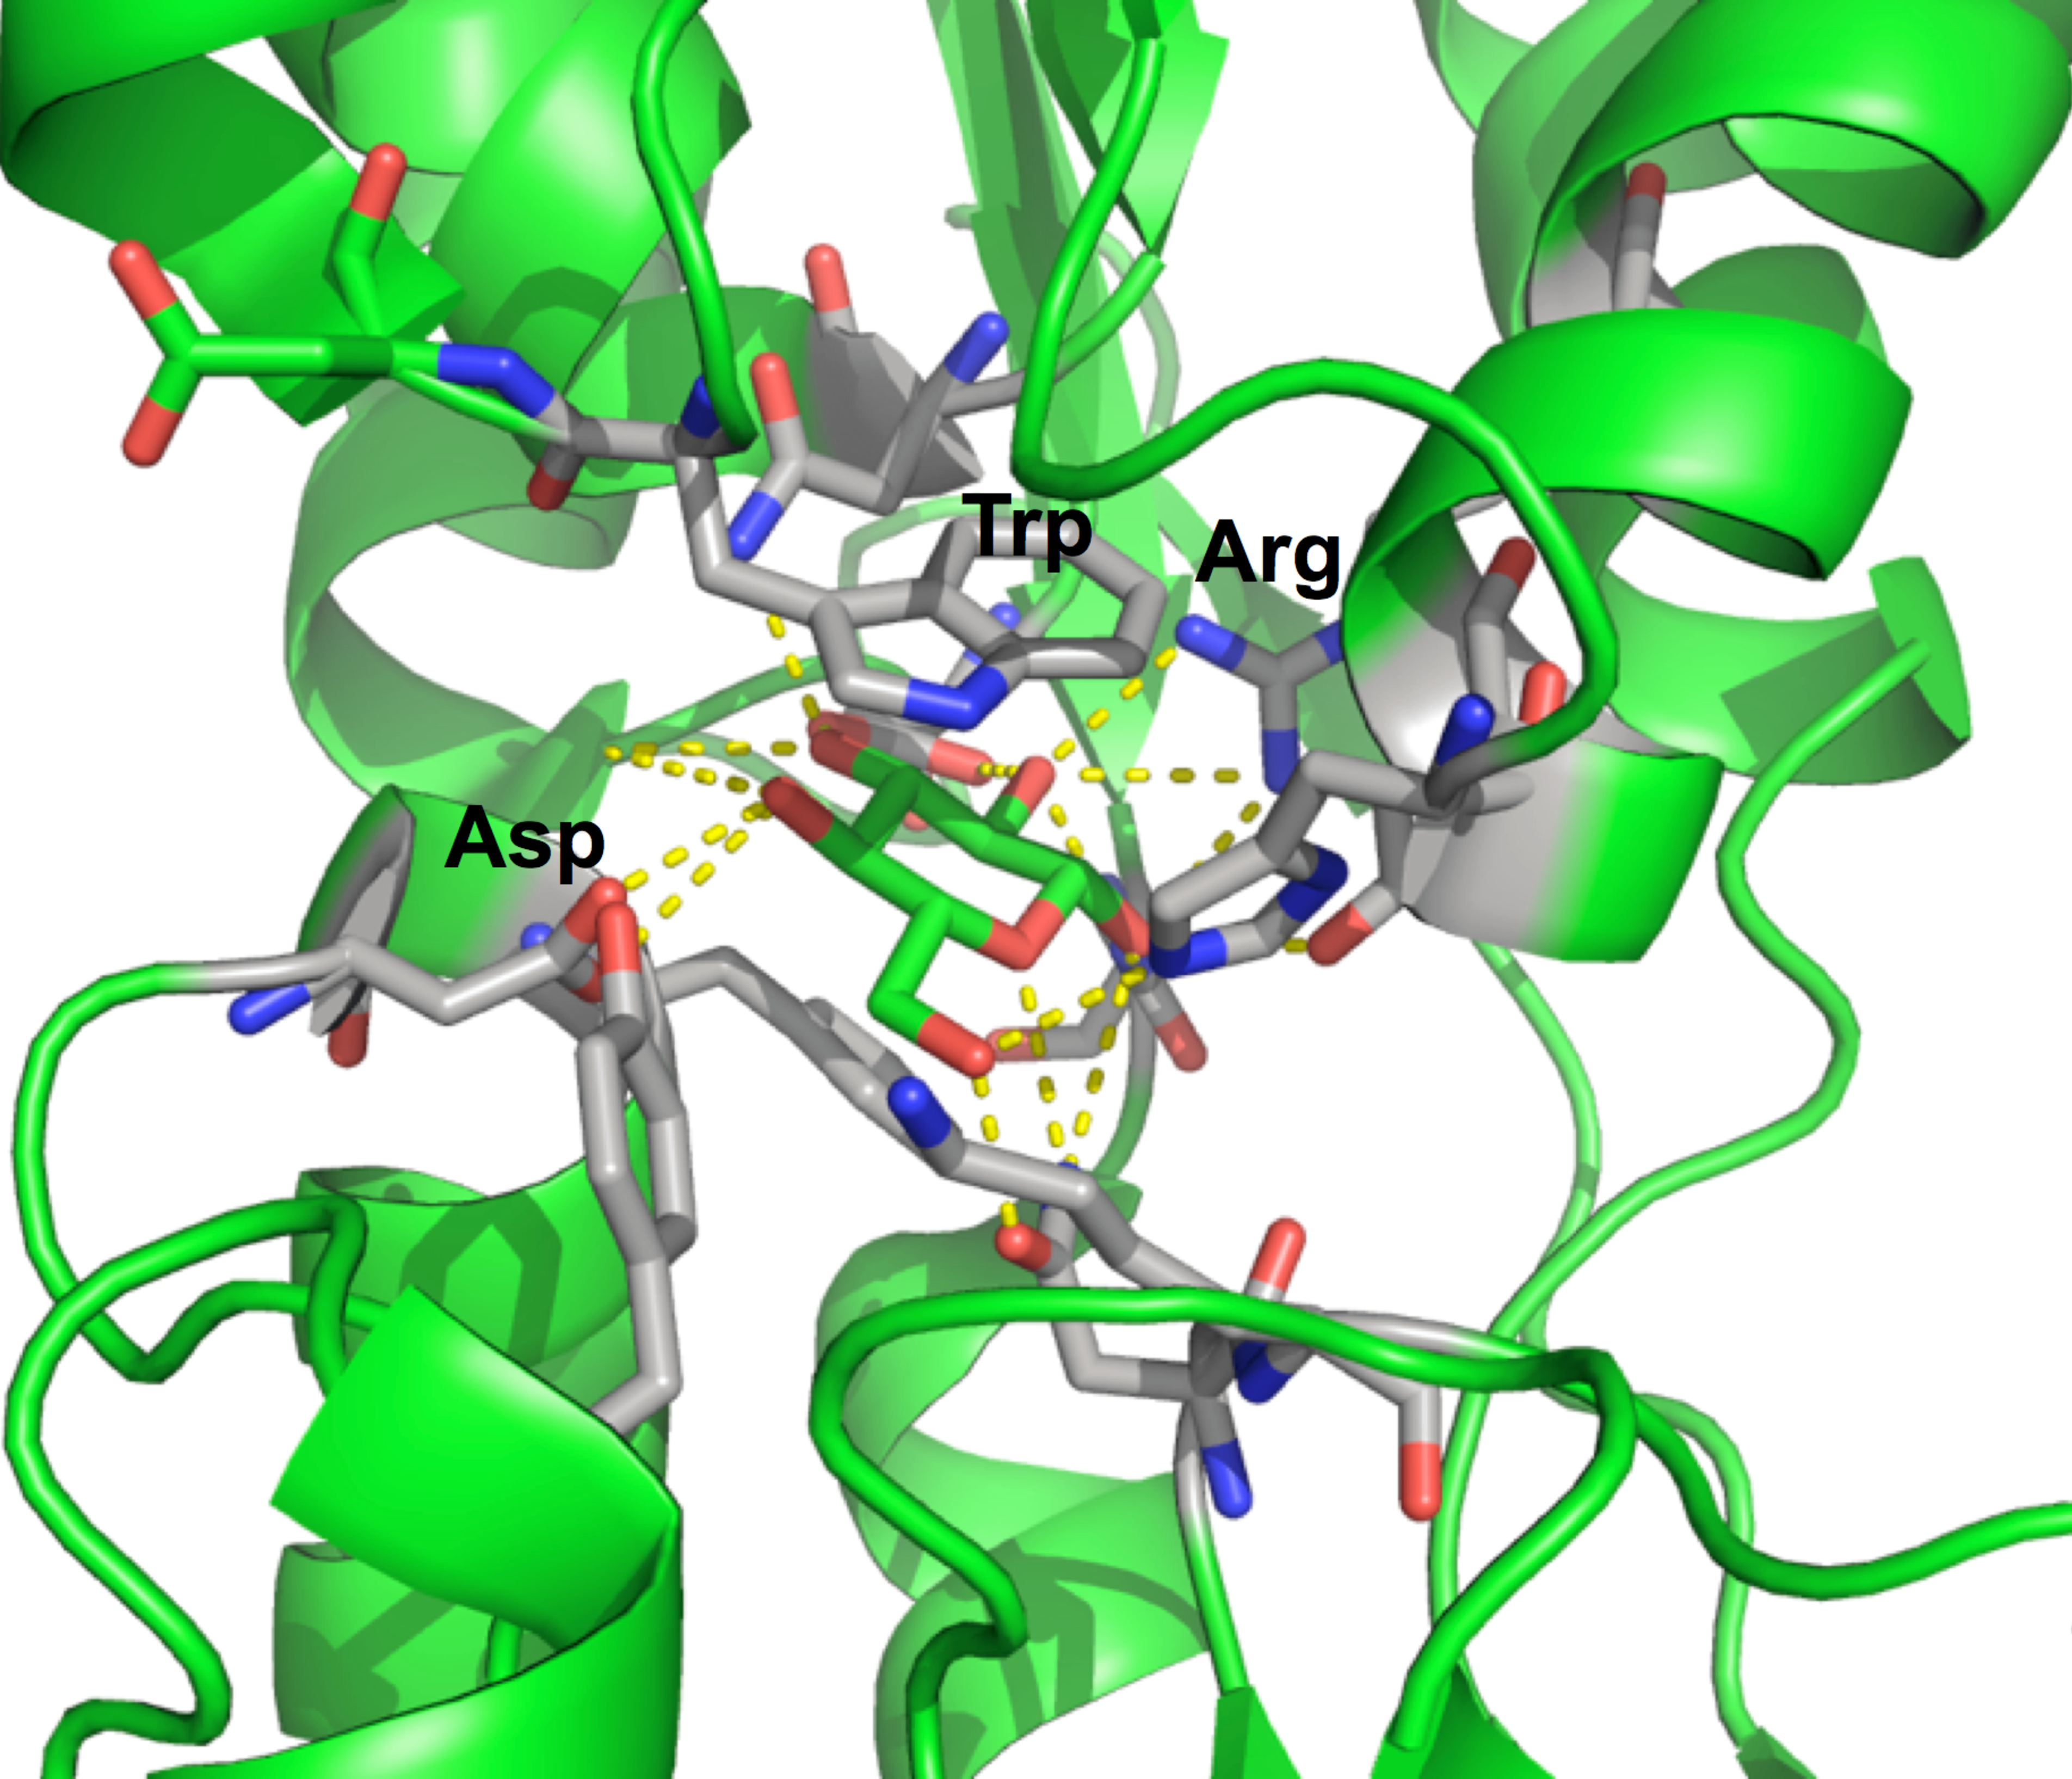
\includegraphics[width=6in]{figures/introduction/sugar_protein_binding.pdf}
  \caption[Sugar protein example]{Example of sugar-lectin mode: glucose binding to galactose chemoreceptor protein (Ref: Vyas, N. et al, 1991; Rendered from PDB ID: 2GP)}
  \label{fig:sugar_protein}
\end{figure}


% \subsection{Role of chirality in drug binding}
% Stereoisomerism is important to the activity of molecules.  It modulates binding to proteins.
% Two types of stereochemistry
% Constitutional isomers - differs in bonding sequences and connectivity
% Stereoisomers - differs in orientation of their atoms in space, but no connectivity differences.
% Definition of chirality [Add schematic] ... etc
% Molecules with chirality have a non-superimposable mirror image, called an enantiomer.
% A carbon molecule with four different groups has chirality.

% From Lemkul, 2012 review of computer simulations of amyloid simulations
% "From a review of the current literature, it is clear that, despite significant progress, a
% comprehensive study of Aβ-small molecule interactions is lacking. Traditional MD simulations
% must include trajectories of sufficient length that are evaluated for convergence, and multiple
% simulations are strongly recommended for statistical reliability. These criteria have not been met
% in some of the studies reviewed here and represent areas of improvement for all investigators to
% consider. Future investigations on this topic should carefully make use of the features of
% docking, traditional MD, and enhanced sampling techniques like metadynamics, DMD, and
% REMD. Such a combined approach, employing a diverse set of Aβ structures as targets for
% docking and MD analysis, will likely shed light on interactions that can be exploited for the
% development of effective anti-aggregation compounds."

\section{Thesis objectives and rationale}
% This is the stuff from my transfer proposal:

% Understanding amyloid inhibition in the context of the framework of traditional enzyme inhibition mechanism
[Challenges of developing small molecule for amyloid inhibition] Structure-based drug discovery approach developed to target folded proteins such as enzymes cannot be directly applied to discovery of small molecules which targets amyloid formation. Because the A$\beta$ amyloid aggregate pathway encompasses a variety of species, some of which are disordered, a single conformation cannot be assumed for binding. Furthermore, structural information of amyloidogenic species lags behind those of enzymes, which tends to be globular proteins amenable for X-ray crystallography. This means that the putative binding sites are not known.  Furthermore, amyloid inhibitors are found to be very weak binders. 
% How do non-specific inhibitors act as a drug? And how do we approach this with MD simulations?
In AD, there is the added challenge of the drug being able to cross the brain barrier, while remaining non-neurotoxic.  What kind of drugs cross the BBB?  Typically hydrophobic drugs.

%     A$\beta$ peptides are completely disordered.  We also do not know what the binding site looks like, where it is located on these structures.

% However, most of these studies were focused on A$\beta$ and large A$\beta$ aggregates,\{Fawzi, 2008 \#553;Esposito, 2008 \#567;Sgourakis, 2007 \#609;Wei, 2006 \#656;Tarus, 2006 \#628 Karsai, 2006 \#658\} and thus, were computationally limited by the complexity of the molecular systems.

% Here describe in detail how I designed my study to circumvent the challenges presented by the amyloid inhibition problem, and the limitations  of MD simulations. At this point, clearly explain and discuss my study design and rationale. 
% (Don't know binding? binding site? which structure does it binding? how does it binding? "binding mechanism")

We don't know if a small-molecule like inositol acts by binding. if ligands bind, and if they bind, we do not know where they bind, and it is experimentally challenging to identify the binding sites using available techniques such as SSNMR, NMR, and X-ray. Although there are some data other there with experimental data, we cannot yet obtain fully atomistic detail on the interactions between the ligands and proteins.

Because amyloid is a group of different species, where the structures of which are largely unknown, we don't know (and we cannot assume) which aggregate species along the amyloid aggregation pathway that inositol may interact with. We want to examine representative species within the aggregation pathway, that is, monomers, disordered oligomers, and fibril like aggregates. Furthermore, we cannot assume putative binding sites - that is these binding sites are not known a priori. Unlike the case with enzymatic inhibition, a single bound molecule is unlikely to inhibit fibrillation. Instead, amyloid aggregates such as fibrils present surfaces for binding.

Although amyloid fibrils of different peptide sequences share the overall cross-beta, there are specific differences in their surface properties due to their amino acid composition. Hence, we look at different species of different peptides.

We took a reductionist approach to solve this problem. Beginning with the simplest model systems for an amyloidogenic peptide, the alanine dipeptide, we systematically examine binding of inositol with systems of both increasing sequence and structural complexity.

% First started with the simplest peptide of relevance, the alanine dipeptide.  We started with the alanine dipeptide to look at backbone interactions. 
We wanted to isolate the problem to something simple to examine the backbone binding mechanism of inositol.  Because inositol had many hydrogen bonding groups, and it is shaped like it is geometrically suited to bind the peptidic backbone. Why did we first choose to look at the backbone?  Because it is the common element in all polypeptides, and the common cross-beta where the backbone of polypeptide chains are organized in the same manner in the structure of amyloid fibrils suggests that backbone plays an important role in amyloid formation.  We examine aggregates of varying sequence and  structural complexity.  By examining a simple beta-sheet forming peptide, (GA)4,  an amyloid inhibitor may bind to a simple amyloidogenic peptide. An illustration of this approach is shown in Figure~\ref{fig:rationale}.

\begin{figure}
  \centering
  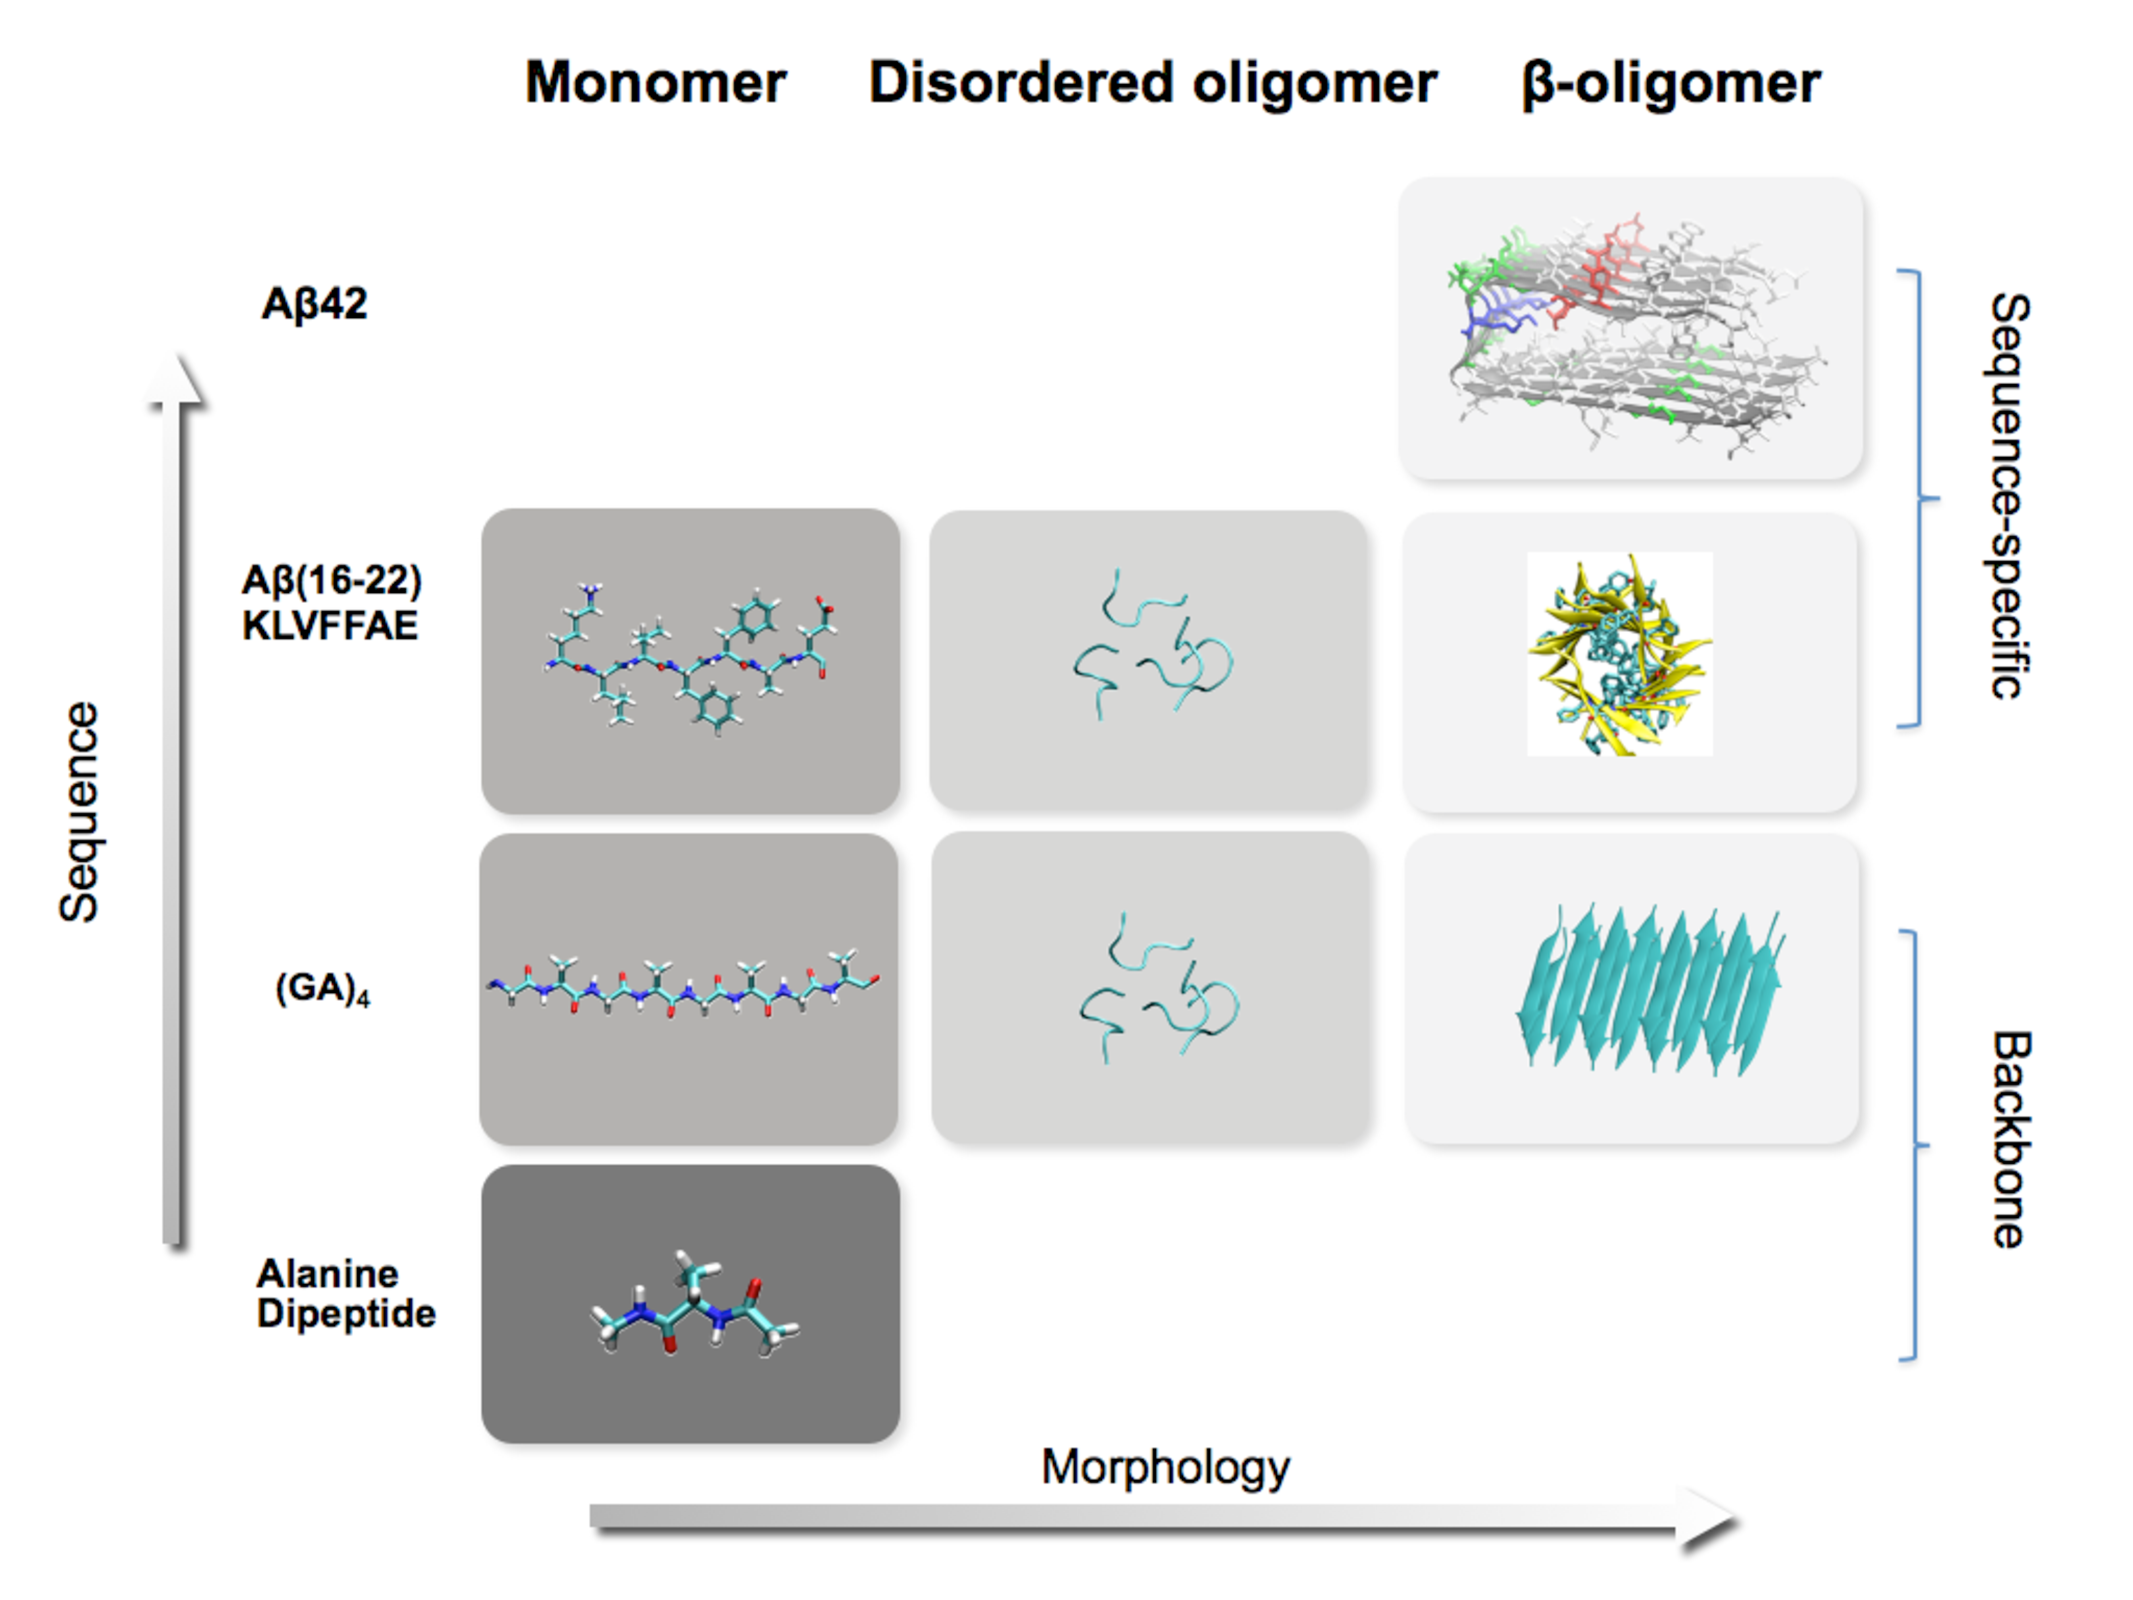
\includegraphics[width=6in]{figures/introduction/matrix.pdf}
  \caption[Rationale]{Shows the progression from small, model systems to larger and structurally more complex systems involving the full-length A$\beta$42 peptide.}
  \label{fig:rationale}
\end{figure}

\subsection{Study Design}

Simulation challenge - The structural disorder of the peptides involved poses a challenge for obtaining converged properties from MD simulations.  To date, few studies have attempted to provide statistically meaningful results pertaining to general mechanisms of protein self-aggregation and amyloid formation. Furthermore, despite the abundance of MD studies of A$\beta$, few studies have systematically examined the mechanism of action of small molecule inhibitors of amyloids

% If you mention brute force ... most scientist in the audience won't understand
For sampling, we exploit conventional MD simulation techniques because simulation approaches used for understanding enzyme-ligand binding is not applicable. Conventional MD simulations were combined with many repeated independent replicas to obtain statistics on the binding equilibria.  We use many repeat simulations - why ? We can observe binding and unbinding events within several nanoseconds.  This is an approach that is typically used to trivially parallelizing simulations to speed up sampling.  Because inositol acts at higher than normal (what do you mean by this) concentrations (in vitro), we were able to approach this problem using a ``bulk" approach, by examining binding between multiple molecules of inositol with different amyloid aggregates.  Inositol's interactions are  weak (but I shouldn't be stating this as an assumption.. because 90% of inositol's interactions may be weak, but the 10% which are not may be the ones that induce its activity).

% Instead, we use conventional MD simulations and repeats of independent simulations to determine the binding modes, and binding equilibria of inositol with amyloidogenic peptides and aggregates of A$\beta$.
\subsection{Hypotheses}
The central hypotheses of the research proposal are as follows:  (1) inositol exerts its effects through direct binding to one or more of the monomeric, aggregated, or fibrillar forms of amyloidogenic peptides and proteins; and (2) binding involves hydrogen bonding interactions with the polypeptidic backbone.

	Two important lines of evidence support the above hypotheses.  First, preliminary experimental data from the McLaurin lab are showing that in addition to Aβ42, inositol can also inhibit superoxide dismutase (an amyloidogenic protein involved in amyotrophic lateral sclerosis), α-synuclein (Parkinson’s disease), and poly-Q (Huntington’s disease) amyloid assemblies in a similar manner to Aβ42 (J. McLaurin unpublished data).  Since all amyloid structures have the cross β-sheet structure in common, their findings suggest that inositol is capable of binding the polypeptide backbone.  Secondly, our own systematic MD study of inositol with alanine dipeptide, a model of the peptidic backbone, has demonstrated that inositol binds to the peptidic backbone through hydrogen bonding interactions (See Section 5.1 below).  

\subsection{Rationale and Specific Aims}
\subsection{Rationale}
	Multiple sources of experimental evidence have demonstrated the existence of species that are morphologically distinct from fibrils in the amyloid aggregation pathway.6, 13, 29  At least two intermediates on pathway to fibril formation have been observed: oligomers and protofibrils. These species together with the monomer and fibrils, constitute a possible pathway by which Aβ aggregates to form fibrils.  
	In order to characterize the molecular mechanism of action of inositol, it is imperative that the interaction of inositol with various aggregate species be examined.  To this end, I will carry out systematic comparative studies of amyloidogenic peptides and their aggregates of increasing sequence and composition complexity and characterize the respective role of specific interactions of inositol with the backbone and sidechains.  Inositols have been shown to have stereochemistry-dependent activity in vitro and in vivo.18, 20  Chiro-inositol is a stereoisomer that was shown to be inactive in inhibiting amyloid formation.  Thus, I will comparatively study chiro- and scyllo-inositol with each of the aggregates in the pathway to determine the stereochemical basis of the activity of inositol.

Specific Aim 1: To determine the effect of inositol on the structure and thermodynamics of the self-aggregation of different amyloidogenic peptides 

Specific Aim 2: To determine the effect of inositol on the kinetics of aggregation

\subsection{Choice of Model Systems}
Following the approach of studying systems of increasing complexity, we have chosen the following peptides and sequences: (1) Alanine Dipeptide; (2) (GA)4; (3) KLVFFAE; (4) SNNFGAIL; (5) Aβ40/42.  Amyloid-forming proteins involved in disease, such as Aβ, Tau (Alzheimer's) or hIAPP (diabetes), are often many residues in length and high in sequence complexity, which renders the collection of meaningful statistics from large-scale computer simulations of these protein aggregates difficult.  However, many of these longer sequences have been found to have shorter segments that preserve the amyloidogenicity and cytotoxicity of the longer parent protein.30, 31 These shorter peptides not only have been shown to retain the physiochemical properties for studying general mechanisms of amyloid formation experimentally, but also are much simpler systems suitable for detailed computational studies.

4.4	Alanine Dipeptide
	Alanine dipeptide (N-acetyl-L-alanine-N'-methylamide or AcAlaNHMe) is a minimalist model of the peptidic backbone with its two backbone dihedral angles (φ,ψ) as its significant degrees of freedom.  The dominant conformations of its conformational equilibrium span all possible dihedral angles representative of α-helices and β-sheets in (Figure 1A).  Due to the simplicity of alanine dipeptide, all relevant local peptidic backbone binding modes of inositol can be explored efficiently computationally.

4.5	GAGAGAGA
	An octamer with repetitive sequence involving only nonpolar side-chains, (GA)4 is the simplest amyloidogenic peptide32 of relevance to study the interaction of inositol with the peptidic backbone. GA is a commonly occurring sequence motif in the β-sheet forming (crystalline) domains of a variety of spider silks.33 The tetramer GAGA is a part of the B. Mori silk fibroin, which is found to contain β-sheet structure.34 The repetitive nature of (GA)4 and its low sequence complexity allow simulations to be computational tractable and thus, permits timescales needed to determine the effects of inositol on amyloid aggregation in a statistically meaningful way.  Finally, the simplicity of (GA)4 allows the detailed examination and dissection of the different possible types of inositol-peptide interactions.  

4.6	KLVFFAE
	The peptide KLVFFAE, a segment spanning residues 16 to 22 of Aβ1-40 and Aβ1-42, has been well studied both experimentally and computationally.35-38 KLVFFAE is the central hydrophobic core thought to be important in full-length Aβ assembly and is affected by four AD causing mutations: A31G (Flemish), E22Q (Dutch), E22K (Italian), and E22G (Arctic).  This peptide not only contains side chains with more bulk, but also those capable of forming charged and aromatic interactions. The protofibrillar structure has been shown by SSNMR to have anti-parallel β-sheet organization with possible parallel stacking of the β-sheets.36  

% 4.7	SNNFGAIL
%	hIAPP(20–27) (SNNFGAIL) is an octameric segment of the 37-amino acid residue hIAPP polypeptide and is both amyloidogenic and cytotoxic.39  Pancreatic amyloid in humans forms through the aggregation of islet amyloid polypeptide (hIAPP).  hIAPP-derived amyloid is found in more than 95% of type II diabetes patients and is believed to be directly involved in the pathogenesis of the disease. The peptide SNNFGAIL is different from KLVFFAE in that it is an amphipathic peptide where SNN is polar and FGAIL is nonpolar.39  Thus, the protofibrillar structure formed will likely have different surface properties despite sharing similar backbone secondary structure.

4.8	Full length Aβ40 or Aβ42
	Inositol does not necessarily act on the shorter peptide models and their aggregates. To address this possibility, I will study inositol with the Aβ peptide and aggregates.  The monomeric, oligomeric, and fibrillar structures of Aβ40 and Aβ42 have been studied both experimentally and computationally.4, 16, 40-45  Thus, I will utilize the structural data available to construct oligomeric and fibrillar species and comparatively analyze the interaction of chiro- and scyllo-inositol with these species.

\section{Thesis Organization}

The first chapter introduces the thesis in the context of the field.  The second chapter introduces the main methods used in the work in the thesis. Chapters 3, 4, and 5 are the results of simulations of inositol with amyloid like peptides and aggregates. Chapter 6 shows work of the general applicability of our methods developed throughout this thesis to MD simulations to understand protein - carbohydrate binding. Chapter 7 provides discussion, suggestions for future work, and perspectives.

\addcontentsline{toc}{section}{Bibliography}
\bibliographystyle{plain}
\bibliography{introduction}

% AD
% Treatment - harder to treat - lack of biochemical understanding of what causes disease, which makes it difficult to develop drugs for; lack of good diagnostic methods because treatment may not be effective at end stages of the disease where brain function won't e able to be rescued.
% Diagnosis - hard to diagnose
% AD is difficult to diagnose.  It is often not apparent that someone has AD until they exhibit symptoms severe enough to interfere with daily life or occupation. 

% Amyloid hypothesis - our best guess at what causes AD and provides the best guess at what we should be targeting. 
% Abeta Amyloid thus far provides the best clue to the molecular basis of AD, and thus a promising pathway to a cure for AD.

% In some individuals without dementia symptoms may have as much plaque as another with severe AD. Synaptic loss can be used as a measure of disease progression. 

% Perhaps use this as a transition into the general discussion of amyloid formation and structure -- not only specific to Abeta.
% Furthermore, amyloid have also been known to play beneficial roles in certain living systems. REF
% Increasing awareness of the amyloid state of proteins, and interest grew in amyloids because of their role in a variety of devastating human diseases.

% Fibrils

% In this section I will talk about how amyloid aggregation is thought to work. Introduce the thermodynamic model for understanding fibril formation.